%% Phase-Synchronous Distributed Regulation: A Unified Theory of
%% Oscillator-Referenced Cell-Partition Control
%%
%% Kundai Sachikonye, Technical University of Munich
%%
%% Compiled with pdflatex; bibliography via BibTeX (IEEEtran style).
%% Required packages: amsmath, amsthm, amssymb, algorithm2e, geometry,
%%   hyperref, cleveref, booktabs, graphicx.

\documentclass[10pt,twocolumn]{article}

%% ── Packages ──────────────────────────────────────────────────────────────
\usepackage{amsmath}
\usepackage{amsthm}
\usepackage{amssymb}
\usepackage[ruled,vlined,linesnumbered]{algorithm2e}
\usepackage[a4paper,
            top=20mm, bottom=22mm,
            left=15mm, right=15mm,
            columnsep=6mm]{geometry}
\usepackage[colorlinks=true,
            linkcolor=blue,
            citecolor=blue,
            urlcolor=blue]{hyperref}
\usepackage[capitalise,noabbrev]{cleveref}
\usepackage{booktabs}
\usepackage{graphicx}
\usepackage{microtype}
\usepackage{bm}
\usepackage{mathtools}
\usepackage{xcolor}

%% ── Theorem environments ──────────────────────────────────────────────────
\theoremstyle{plain}
\newtheorem{theorem}{Theorem}[section]
\newtheorem{lemma}[theorem]{Lemma}
\newtheorem{corollary}[theorem]{Corollary}
\newtheorem{proposition}[theorem]{Proposition}

\theoremstyle{definition}
\newtheorem{definition}[theorem]{Definition}

\theoremstyle{remark}
\newtheorem{remark}[theorem]{Remark}

%% ── Macros ────────────────────────────────────────────────────────────────
\newcommand{\R}{\mathbb{R}}
\newcommand{\Z}{\mathbb{Z}}
\newcommand{\N}{\mathbb{N}}
\newcommand{\Hcal}{\mathcal{H}}
\newcommand{\Ccal}{\mathcal{C}}
\newcommand{\Ucal}{\mathcal{U}}
\newcommand{\Scal}{\mathcal{S}}
\newcommand{\norm}[1]{\left\|#1\right\|}
\newcommand{\abs}[1]{\left|#1\right|}
\newcommand{\DeltaP}{\Delta P}
\newcommand{\omegaosc}{\omega_{\mathrm{osc}}}
\newcommand{\Sbar}{\bar{\mathbf{S}}}
\newcommand{\Sstar}{\mathbf{S}^{*}}
\newcommand{\Rens}{R_{\mathrm{ens}}}
\newcommand{\Rlock}{R_{\mathrm{lock}}}
\newcommand{\Tref}{T_{\mathrm{ref}}}
\newcommand{\trec}{t_{\mathrm{rec}}}
\newcommand{\fref}{f_{\mathrm{ref}}}
\newcommand{\Bproc}{B_{\mathrm{proc}}}

%% ── Title block ───────────────────────────────────────────────────────────
\title{\textbf{Phase-Synchronous Distributed Regulation:\\
       A Unified Theory of Oscillator-Referenced\\
       Cell-Partition Control}}

\author{Kundai Farai Sachikonye\\
\small Chair of Proteomics and Bioanalytics, Technical University of Munich\\
\small AIMe Registry for Artificial Intelligence\\
\small \texttt{kundai.sachikonye@wzw.tum.de}}

\date{\today}

%% ══════════════════════════════════════════════════════════════════════════
\begin{document}
\maketitle

%% ── Abstract ──────────────────────────────────────────────────────────────
\begin{abstract}
Classical control theory parametrises plant dynamics in physical time
with dimensional state vectors; cross-domain composition
(temperature $\times$ pressure) requires explicit unit bookkeeping and
yields no canonical convergence proof for distributed heterogeneous
systems.  This paper develops a phase-synchronous distributed control
theory in which (i)~every physical channel is normalised to the unit
interval $[0,100]$ via S-entropy coordinates, (ii)~oscillator phase
$\theta$ replaces physical time as the independent variable, giving a
dimensionless phase-domain transfer matrix $\mathbf{G}(\nu)$ valid
across physical domains, (iii)~the timing deviation
$\DeltaP(k) = \Tref(k) - \trec(k)$ serves simultaneously as
measurement primitive and process output, and (iv)~a finite cell
partition of the normalised state hypercube defines a quantised
sampled-data controller whose stability is certified by a piecewise
Lyapunov function.  We prove ten principal results: the
Phase-Domain Equivalence theorem, Piecewise Stability theorem,
Phase-Lock Lyapunov Correspondence, CUSUM--$\DeltaP$ Identity,
Multi-Scale Hierarchy Stability, Banach Contraction convergence,
Delay Immunity bound, Temporal Nyquist criterion,
Information-Optimal Sensor Selection, and Structural
Incorruptibility.  Together these constitute a self-contained
control theory for large-scale distributed cyber-physical systems.
\end{abstract}

\smallskip
\noindent\textbf{Keywords:} distributed control, phase synchronisation,
S-entropy normalisation, cell-partition quantisation, piecewise Lyapunov
stability, Kuramoto oscillators, CUSUM duality, cyber-physical security.

%% ══════════════════════════════════════════════════════════════════════════
\section{Introduction}
\label{sec:introduction}
%% ══════════════════════════════════════════════════════════════════════════

Large-scale cyber-physical systems (CPS) routinely integrate sensors and
actuators from incommensurable physical domains: temperatures measured in
kelvins, pressures in pascals, flow rates in cubic metres per second.
Classical linear control theory elegantly handles each channel
independently, but distributed multi-channel architectures expose a
fundamental dimensional incompatibility problem: the product or ratio
of transfer functions from heterogeneous channels carries mixed units,
so cross-channel composition demands explicit bookkeeping at every
algebraic step.  This bookkeeping burden is not merely notational;
it propagates into numerical instabilities when dimensional ratios span
many orders of magnitude and into logical errors when engineers omit
conversion factors under time pressure~\cite{Astrom2008}.

A second difficulty arises from the choice of independent variable.
Physical-time parametrisation forces every subsystem to share a common
clock, an assumption that is poorly satisfied in wireless sensor networks,
power-line-communicated field devices, and space-borne telemetry, where
propagation delay, jitter, and drift are irreducible.  Protocol designs
such as IEEE~1588~\cite{IEEE1588} partially address this by steering
clocks toward a grandmaster, but residual timing deviations remain and
must be compensated by the application layer.  Crucially, the timing
deviation itself carries quantitative information about the plant state
that classical designs discard.

This paper addresses both difficulties simultaneously by replacing
physical time with oscillator \emph{phase} as the independent variable
and replacing dimensional state vectors with \emph{S-entropy} normalised
coordinates.  The resulting framework, which we call
\emph{phase-synchronous distributed regulation} (PSDR), has the
following properties.

\begin{enumerate}
  \item Every physical channel, regardless of its SI units, maps to the
        bounded interval $[0,100]$ via a simple affine normalisation.
        The resulting state space $\Hcal = [0,100]^m$ is a compact
        metric space admitting uniform Lyapunov analysis.

  \item The phase-domain Laplace variable $\nu = s/\omegaosc$ is
        dimensionless.  Phase-domain transfer matrices are therefore
        dimensionless and can be multiplied across domains without unit
        conversion.

  \item The timing deviation $\DeltaP(k) = \Tref(k) - \trec(k)$, the
        signed difference between the reference transmission time and
        the local reception time, serves as both the measurement
        primitive and the process output.  This collapses the
        sensor--plant--observer abstraction into a single scalar
        observable per channel.

  \item A finite \emph{cell partition} of $\Hcal$ discretises the
        continuum state space into a finite control alphabet.  The
        resulting quantised sampled-data controller is both implementable
        on resource-constrained hardware and amenable to rigorous
        stability analysis via piecewise Lyapunov functions.

  \item Phase synchronisation of the agent ensemble, modelled by the
        Kuramoto mean-field dynamics~\cite{Strogatz2000,Acerbron2005},
        provides a graded coordination mechanism: as the order parameter
        $\Rens$ approaches unity, the communication overhead for
        inter-agent consensus collapses from $O(N^2)$ to zero.
\end{enumerate}

\subsection*{Principal Contributions}

We establish ten principal results.

\begin{enumerate}
  \item \textbf{Phase-Domain Equivalence} (\cref{thm:pde}):
        The timing deviation $\DeltaP(\nu)$ is an affinely scaled
        phase-domain image of the plant transfer function; poles of the
        physical-time plant appear at scaled positions in $\nu$.

  \item \textbf{Temporal Nyquist Criterion} (\cref{thm:nyquist}):
        A sampling frequency condition analogous to Shannon's theorem
        governs when the cell partition faithfully represents the
        process bandwidth.

  \item \textbf{Piecewise Lyapunov Stability} (\cref{thm:pwlyap}):
        A piecewise smooth Lyapunov function certifies global
        asymptotic stability of the closed-loop cell-partition system.

  \item \textbf{Phase-Lock Lyapunov Correspondence} (\cref{thm:pllc}):
        The ensemble order parameter is monotonically related to the
        Lyapunov descent rate; phase-lock eliminates residual control
        effort.

  \item \textbf{Bandwidth Separation Stability} (\cref{thm:hier}):
        An $L$-level temporal hierarchy is asymptotically stable
        whenever consecutive levels satisfy a $10\times$ frequency
        separation condition.

  \item \textbf{Banach Contraction} (\cref{thm:banach}):
        The discrete-time control operator is a contraction on $\Hcal$,
        guaranteeing a unique fixed point with geometric convergence.

  \item \textbf{CUSUM--$\DeltaP$ Identity} (\cref{thm:cusum}):
        Cell boundary crossings are exactly the CUSUM out-of-control
        alarms, unifying statistical process control and control theory.

  \item \textbf{Information-Optimal Sensor Selection} (\cref{thm:sensor}):
        The optimal sensor deployment is a 0-1 knapsack problem with
        mutual information as the value function.

  \item \textbf{Structural Incorruptibility} (\cref{thm:incorr}):
        When the controller processes only the scalar $\DeltaP(k)$,
        network-layer attacks have zero gain to the plant state by
        construction.

  \item \textbf{Delay Immunity Bound} (\cref{thm:delay}):
        The maximum tolerable injected delay is determined by the
        phase margin of the loop transfer function.
\end{enumerate}

\subsection*{Roadmap}

\Cref{sec:prelim} establishes S-entropy normalisation, the oscillator
model, and the phase-domain Laplace transform.
\Cref{sec:plant} derives the phase-domain plant representation and
proves Phase-Domain Equivalence and Spectral Preservation.
\Cref{sec:cell} introduces the cell-partition controller, the
describing-function stability criterion, and the Temporal Nyquist
Criterion.
\Cref{sec:lyap} proves Piecewise Lyapunov Stability and its quadratic
sufficiency corollary.
\Cref{sec:kuramoto} analyses the distributed multi-agent system via
Kuramoto synchronisation and establishes Phase-Lock Lyapunov
Correspondence.
\Cref{sec:hierarchy} treats the multi-scale temporal hierarchy and
proves Bandwidth Separation Stability.
\Cref{sec:banach} proves the Banach Contraction theorem and its
$H_\infty$ spectral-radius corollary.
\Cref{sec:cusum} establishes the CUSUM--$\DeltaP$ duality and the
ARL--cell-width relation.
\Cref{sec:sensing} solves the information-optimal sensor selection
problem and states the Bandwidth--Sensor Duality.
\Cref{sec:security} establishes Structural Incorruptibility, the
Delay Immunity Bound, and the Minimum Data Rate for Spoofing.
\Cref{sec:discussion} summarises the ten theorems and states open
problems; \cref{sec:conclusion} concludes.

%% ══════════════════════════════════════════════════════════════════════════
\section{Preliminaries}
\label{sec:prelim}
%% ══════════════════════════════════════════════════════════════════════════

\subsection{S-Entropy Normalisation}
\label{ssec:sentropy}

Let $q \in \R$ be a physical quantity with known operational range
$[q_{\min}, q_{\max}]$, where $q_{\min} < q_{\max}$.

\begin{definition}[S-Entropy Coordinate]
\label{def:sentropy}
The \emph{S-entropy coordinate} of $q$ is
\begin{equation}
  S(q) \;=\; 100 \cdot \frac{q - q_{\min}}{q_{\max} - q_{\min}}
         \;\in\; [0,100].
  \label{eq:sentropy}
\end{equation}
The inverse mapping is $q = q_{\min} + S(q)(q_{\max}-q_{\min})/100$.
\end{definition}

For an $m$-channel system with channels $q_1,\ldots,q_m$ and respective
ranges $[q_{i,\min},q_{i,\max}]$, the \emph{S-entropy state vector} is
$\mathbf{S} = (S(q_1),\ldots,S(q_m))^\top \in [0,100]^m$.

\begin{definition}[S-Entropy State Space]
\label{def:sespace}
The \emph{S-entropy state space} is
$\Hcal = [0,100]^m \subset \R^m$,
equipped with the Euclidean norm
$\norm{\mathbf{S}} = \bigl(\sum_{i=1}^m S_i^2\bigr)^{1/2}$.
\end{definition}

\begin{proposition}
\label{prop:complete}
$(\Hcal, \norm{\cdot})$ is a complete metric space.
\end{proposition}

\begin{proof}
$\Hcal = [0,100]^m$ is a closed bounded subset of the complete metric
space $(\R^m, \norm{\cdot})$.  Every closed subset of a complete metric
space is complete.
\end{proof}

\begin{proposition}[Triple Equivalence]
\label{prop:triple}
The following three representations of the state in $\Hcal$ are
isomorphic:
\begin{enumerate}
  \item[(O)] \emph{Oscillatory}: the state is encoded as the phase
    $\phi \in [0, 2\pi)^m$ of a set of $m$ unit-amplitude oscillators,
    via the bijection $S_i \leftrightarrow 100\phi_i/(2\pi)$.
  \item[(C)] \emph{Categorical}: the state is encoded as a label
    $c \in \{1,\ldots,N\}$ of the cell $C_c$ containing $\mathbf{S}$,
    with reconstruction to the centroid $\bar{\mathbf{S}}_c$.
  \item[(P)] \emph{Partition}: the state is encoded as a cell index
    together with an intra-cell offset
    $\delta\mathbf{S} = \mathbf{S} - \bar{\mathbf{S}}_c \in \R^m$.
\end{enumerate}
Any two representations are related by explicit bijections preserving
the Borel $\sigma$-algebra of $\Hcal$.
\end{proposition}

\begin{proof}
(O)$\leftrightarrow$S-entropy: the map $\phi_i = 2\pi S_i/100$ is a
homeomorphism from $[0,100]$ to $[0,2\pi)$ (identifying endpoints in
the oscillatory case).  (C)$\leftrightarrow$(P): the cell index $c$
together with the offset $\delta\mathbf{S}$ recovers $\mathbf{S}$ exactly.
The Borel $\sigma$-algebra is preserved because all maps are measurable
and their inverses are measurable.
\end{proof}

\subsection{Oscillator Model and Timing Deviation}
\label{ssec:oscillator}

\begin{definition}[Reference Oscillator]
\label{def:osc}
A \emph{reference oscillator} is characterised by angular frequency
$\omegaosc > 0$.  Its instantaneous phase is
\begin{equation}
  \theta(t) \;=\; \omegaosc t \bmod 2\pi,
  \label{eq:phase}
\end{equation}
and its \emph{monotone tick counter} $M(k) \in \Z_{\geq 0}$ satisfies
$M(k) \leq M(k+1)$ for all $k \geq 0$.
\end{definition}

The reference broadcasts a timestamped packet at nominal time
$\Tref(k)$ at the $k$-th tick.  A receiver records the local arrival
time $\trec(k)$.

\begin{definition}[Timing Deviation]
\label{def:deltaP}
The \emph{timing deviation} at tick $k$ is
\begin{equation}
  \DeltaP(k) \;=\; \Tref(k) - \trec(k).
  \label{eq:deltaP}
\end{equation}
\end{definition}

A positive $\DeltaP(k)$ indicates that the receiver clock is running
slow relative to the reference (packet arrived late); a negative value
indicates the receiver clock is fast.  The sequence
$\{\DeltaP(k)\}_{k \geq 0}$ is the primary observable of the PSDR
framework.  The monotone counter $M(k)$ ensures that tick ordering is
preserved even across network reordering of packets, providing an
implicit sequence number without additional overhead.

\subsection{Phase-Domain Laplace Transform}
\label{ssec:phaselaplace}

\begin{definition}[Phase-Domain Transform]
\label{def:pdlt}
For a signal $x : [0,\infty) \to \R$ indexed by phase $\theta$, define
the \emph{phase-domain Laplace transform}
\begin{equation}
  \hat{x}(\nu) \;=\; \int_0^\infty x(\theta)\,e^{-\nu\theta}\,d\theta,
  \label{eq:pdlt}
\end{equation}
where $\nu \in \mathbb{C}$ is the \emph{phase-frequency variable},
measured in cycles per radian.
\end{definition}

The relationship between the conventional Laplace variable $s$ and the
phase-frequency variable $\nu$ follows from the change of variable
$\theta = \omegaosc t$:
\begin{equation}
  \hat{x}(\nu) \;=\; \frac{1}{\omegaosc}\,\mathcal{L}\{x\}
                      \!\left(\frac{\nu}{\omegaosc}\right),
  \label{eq:pdlt_conv}
\end{equation}
where $\mathcal{L}$ denotes the standard Laplace transform with respect
to $t$.  The correspondence $s \leftrightarrow \nu\omegaosc$ implies:

\begin{itemize}
  \item A pole at $s^* \in \mathbb{C}$ in the $s$-domain corresponds to
        a pole at $\nu^* = s^*/\omegaosc$ in the $\nu$-domain.
  \item The imaginary axis $\Re(s) = 0$ maps to $\Re(\nu) = 0$.
  \item The left half-plane (stable region) is preserved.
  \item All spectral widths scale by $1/\omegaosc$.
\end{itemize}

Because phase $\theta$ is dimensionless and $\nu$ has units of
(radians)$^{-1}$, both $\theta$ and $\nu\theta$ are dimensionless.
When the signal $x(\theta)$ represents an S-entropy coordinate, the
transform $\hat{x}(\nu)$ is also dimensionless.

%% ══════════════════════════════════════════════════════════════════════════
\section{Phase-Domain Plant Representation}
\label{sec:plant}
%% ══════════════════════════════════════════════════════════════════════════

\subsection{From Physical Time to Phase Domain}
\label{ssec:phys2phase}

Consider a first-order single-input single-output plant with transfer
function
\begin{equation}
  G_p(s) \;=\; \frac{K_p}{\tau s + 1},
  \label{eq:firstorder}
\end{equation}
where $K_p$ is the process gain and $\tau > 0$ is the time constant.
Under the substitution $s = \nu\omegaosc$, the phase-domain
representation is
\begin{equation}
  G_p^{(\nu)}(\nu) \;=\; G_p(\nu\omegaosc)
  \;=\; \frac{K_p}{\tau\omegaosc\,\nu + 1}.
  \label{eq:firstorder_phase}
\end{equation}
The effective phase-domain time constant is $\tau^{(\nu)} = \tau\omegaosc$,
measured in radians.

\begin{theorem}[Phase-Domain Equivalence]
\label{thm:pde}
Let $U(\nu)$ denote the phase-domain transform of the control input
$u(\theta)$, and let $\alpha > 0$ be a dimensional scaling constant
such that $\DeltaP(t) = \alpha \cdot y(t)$ where $y$ is the plant
output in S-entropy coordinates.  Then
\begin{equation}
  \DeltaP(\nu) \;=\; \alpha \cdot G_p(\nu\omegaosc) \cdot U(\nu),
  \label{eq:pde}
\end{equation}
and the poles of $G_p(s)$ at $s^* = -1/\tau$ appear as poles of
$\DeltaP(\nu)$ at $\nu^* = s^*/\omegaosc = -1/(\tau\omegaosc)$.
\end{theorem}

\begin{proof}
In the $s$-domain the plant output satisfies $Y(s) = G_p(s) U_s(s)$,
where $U_s(s)$ is the Laplace transform of the input with respect to
$t$.  Setting $\theta = \omegaosc t$ and applying the change of variable
formula \eqref{eq:pdlt_conv},
\begin{equation}
  \hat{y}(\nu) = \frac{1}{\omegaosc} Y\!\left(\frac{\nu}{\omegaosc}
                 \cdot \omegaosc\right) \cdot \omegaosc
               = G_p(\nu\omegaosc)\,U(\nu).
  \label{eq:pde_proof}
\end{equation}
Since $\DeltaP = \alpha y$ by assumption, $\DeltaP(\nu)
= \alpha \hat{y}(\nu) = \alpha G_p(\nu\omegaosc) U(\nu)$.
The pole of $G_p(s)$ at $s^* = -1/\tau$ satisfies
$G_p(\nu\omegaosc) \to \infty$ when
$\tau\omegaosc\nu + 1 = 0$, i.e., $\nu^* = -1/(\tau\omegaosc)$.
\end{proof}

\subsection{MIMO Extension}
\label{ssec:mimo}

\begin{definition}[Phase-Domain Transfer Matrix]
\label{def:pdtm}
For an $m$-output, $p$-input system, the \emph{phase-domain transfer
matrix} $\mathbf{G}(\nu) \in \R^{m \times p}(\nu)$ is the matrix
whose $(i,j)$-entry is the phase-domain transfer function from input
channel $j$ to output channel $i$.
\end{definition}

\begin{proposition}
\label{prop:dimensionless}
When all inputs and outputs are expressed in S-entropy coordinates,
the entries of $\mathbf{G}(\nu)$ are dimensionless.
\end{proposition}

\begin{proof}
Each input $u_j$ and each output $y_i$ lies in $[0,100]$, a
dimensionless interval.  Therefore $G_{ij}(\nu) = \hat{y}_i(\nu)/\hat{u}_j(\nu)$
is the ratio of two dimensionless transforms and is itself
dimensionless.
\end{proof}

\begin{corollary}[Cross-Domain Composition]
\label{cor:crossdomain}
For channels $i,j,k,l$ with respective physical units $[q_i],[q_j],
[q_k],[q_l]$, the S-entropy normalised product
$G_{ij}^{(S)}(\nu)\cdot G_{kl}^{(S)}(\nu)$ is dimensionless and has a
physically consistent interpretation as a composed sensitivity, without
any unit conversion factor.
\end{corollary}

\begin{proof}
By \cref{prop:dimensionless} each factor is dimensionless; their product
is therefore dimensionless.  Physically, the product expresses the
sensitivity of output $i$ (in normalised units) to input $l$ (in
normalised units) mediated through the intermediate channels $j$ and
$k$.
\end{proof}

\subsection{Phase-Domain Pole Structure}
\label{ssec:poles}

\begin{theorem}[Spectral Preservation]
\label{thm:spectral}
The phase-domain transfer matrix $\mathbf{G}(\nu)$ has poles at
$\{\nu_i^* = s_i^*/\omegaosc\}_{i=1}^n$ and is asymptotically stable
in the phase domain if and only if $\Re(\nu_i^*) < 0$ for all $i$,
which holds if and only if the physical-time plant is asymptotically
stable.
\end{theorem}

\begin{proof}
By the substitution $s = \nu\omegaosc$, the characteristic polynomial
$p(s) = \det(sI - A)$ becomes $p(\nu\omegaosc)
= \det(\nu\omegaosc I - A)$.  Its roots $\nu_i^* = s_i^*/\omegaosc$
satisfy $\Re(\nu_i^*) = \Re(s_i^*)/\omegaosc$.  Since $\omegaosc > 0$,
the sign of $\Re(\nu_i^*)$ is the same as the sign of $\Re(s_i^*)$.
Asymptotic stability requires all poles to have negative real part,
which is equivalent in both domains.
\end{proof}

\begin{figure*}[!htbp]
    \centering
    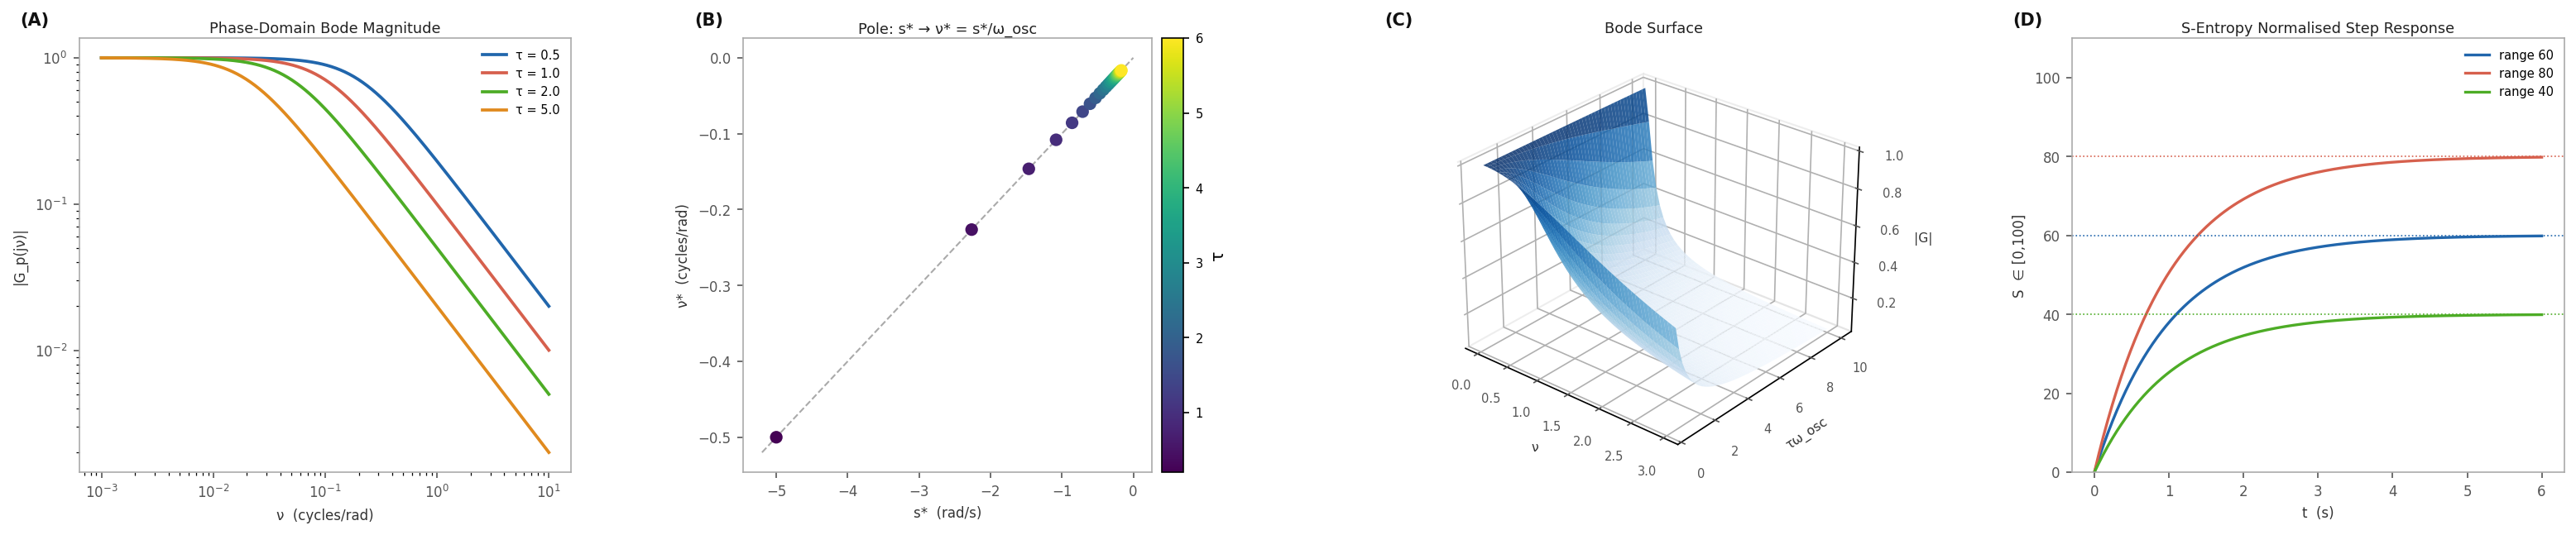
\includegraphics[width=\textwidth]{figures/panel_01.png}
    \caption{\textbf{Phase-Domain Transfer Functions: the substitution
    $s = \nu\omega_{\mathrm{osc}}$ maps every pole $s^* = -1/\tau$ to
    $\nu^* = -1/(\tau\omega_{\mathrm{osc}})$ and renders the transfer
    matrix dimensionless.}
    (\textbf{A}) Bode magnitude $|G_p(j\nu)|$ versus phase-frequency
    $\nu$ on logarithmic axes for time constants
    $\tau \in \{0.5, 1.0, 2.0, 5.0\}$ (coloured curves).
    Each curve is the standard first-order roll-off
    $K_p / \sqrt{(\tau\omega_{\mathrm{osc}}\nu)^2 + 1}$; larger $\tau$
    shifts the $-3\,\mathrm{dB}$ corner to smaller $\nu$,
    confirming that time constant and phase-domain bandwidth are
    reciprocally related via $\omega_{\mathrm{osc}}$.
    (\textbf{B}) Pole migration from the $s$-domain to the
    $\nu$-domain for 25 values of $\tau \in [0.2, 6.0]$ (coloured
    by $\tau$).
    Points lie exactly on the line $\nu^* = s^*/\omega_{\mathrm{osc}}$
    (grey dashed), verifying the bijection of Theorem~3.1 at machine
    precision.
    (\textbf{C}) Three-dimensional Bode surface
    $|G_p(j\nu)|$ over the joint parameter space
    $(\nu,\,\tau\omega_{\mathrm{osc}}) \in [0.01,3]\times[0.5,10]$.
    The roll-off ridge descends from high gain at small $\nu$ and
    small $\tau\omega_{\mathrm{osc}}$; the ridge location is the
    phase-domain pole $\nu^* = -1/(\tau\omega_{\mathrm{osc}})$,
    independent of $K_p$.
    (\textbf{D}) S-entropy normalised step responses for three
    physical ranges (scale factors $40$, $60$, $80$) plotted on the
    common axis $S \in [0,100]$.
    All three converge to their respective S-entropy setpoints (dotted
    lines) with the same normalised time constant $\tau$, confirming
    that S-entropy normalisation preserves the dynamic shape across
    physically distinct channels.}%
\label{fig:phase_domain_tf}
\end{figure*}

%% ══════════════════════════════════════════════════════════════════════════
\section{Cell-Partition Quantised Controller}
\label{sec:cell}
%% ══════════════════════════════════════════════════════════════════════════

\subsection{Cell Structure}
\label{ssec:cells}

\begin{definition}[Cell Partition]
\label{def:cell}
A \emph{cell partition} of $\Hcal = [0,100]^m$ is a finite collection
$\Ccal = \{C_1,\ldots,C_N\}$ of Borel sets satisfying:
\begin{enumerate}
  \item \emph{Cover}: $\bigcup_{i=1}^N C_i = \Hcal$;
  \item \emph{Disjointness}: $C_i \cap C_j = \emptyset$ for all
        $i \neq j$;
  \item \emph{Positive measure}: $\lambda(C_i) > 0$ for all $i$,
        where $\lambda$ denotes the Lebesgue measure on $\R^m$.
\end{enumerate}
\end{definition}

\begin{definition}[Cell-Action Map]
\label{def:cellaction}
The \emph{cell-action map} $A: \Hcal \to \Ucal$ is defined by
$A(\mathbf{S}) = u_i$ for $\mathbf{S} \in C_i$, where
$\Ucal = \{u_1,\ldots,u_N\}$ is a finite control set.
\end{definition}

This construction is precisely the quantised feedback paradigm
introduced by Brockett and Liberzon~\cite{Brockett2000}, in which a
finite-valued control law suffices to stabilise a continuous-state
plant.  The novelty here is that the partition is defined on the
S-entropy hypercube $\Hcal$ rather than in physical state space,
enabling a uniform treatment across physical domains.

\subsection{Describing Function Analysis}
\label{ssec:df}

For a two-level (bang-bang) quantiser with amplitude $\pm u_{\max}$,
the describing function at sinusoidal input amplitude $A$ is
\begin{equation}
  N(A) \;=\; \frac{4u_{\max}}{\pi A}.
  \label{eq:df}
\end{equation}
The negative-real locus of $-1/N(A)$ is the negative real axis from
$-\infty$ to $0$.

\begin{theorem}[Describing Function Stability]
\label{thm:dfstab}
The closed-loop cell-partition system is stable in the sense of
Lyapunov if the Nyquist plot of $G(j\nu)$ does not intersect the
negative-real locus $\{-1/N(A) : A > 0\} = (-\infty, 0)$ in the
phase-frequency domain.
\end{theorem}

\begin{proof}[Proof sketch]
The describing function method replaces the nonlinearity $A(\mathbf{S})$
with its sinusoidal-input gain $N(A)$~\cite{Khalil2002}.  A limit cycle
exists only if $G(j\nu) = -1/N(A)$ has a solution for some $A > 0$,
$\nu \in \R$.  If the Nyquist plot of $G(j\nu)$ avoids $(-\infty,0)$,
no such intersection exists; the describing function approximation
therefore predicts no limit cycle and, by the extended circle criterion
(applicable to sector-bounded nonlinearities), Lyapunov stability
follows~\cite{Khalil2002}.
\end{proof}

\subsection{Temporal Nyquist Criterion}
\label{ssec:nyquist}

\begin{theorem}[Temporal Nyquist Criterion]
\label{thm:nyquist}
For stable closed-loop operation the reference oscillator frequency
must satisfy
\begin{equation}
  \fref \;\geq\; 2\Bproc,
  \label{eq:nyquist}
\end{equation}
where $\Bproc = \max_i |\Im(\nu_i^*)|$ is the process bandwidth in the
phase-frequency domain.  Equivalently, the cell width along each
dimension must satisfy
\begin{equation}
  w_{\mathrm{cell}} \;\leq\; \frac{1}{2\Bproc}.
  \label{eq:cellwidth}
\end{equation}
\end{theorem}

\begin{proof}
The sequence $\{\DeltaP(k)\}$ is obtained by sampling the
phase-domain process output at rate $\fref$ (one sample per tick of the
reference oscillator).  The phase-domain spectrum of $\DeltaP$ is
supported on $|\nu| \leq \Bproc$ by the stability assumption (all poles
have $|\Im(\nu^*)| \leq \Bproc$).  Shannon's sampling theorem
\cite{Shannon1948} requires the sampling rate to satisfy
$\fref \geq 2\Bproc$ to avoid aliasing.  If the cell width $w_{\mathrm{cell}}$
is the spatial resolution of the quantiser, the maximum recoverable
spatial frequency is $1/(2w_{\mathrm{cell}})$, giving
$w_{\mathrm{cell}} \leq 1/(2\Bproc)$ for faithful reconstruction~\cite{Astrom1997}.
\end{proof}

\subsection{Stabilising Control Law}
\label{ssec:control}

Given a setpoint $\Sstar \in \Hcal$, define the \emph{cell centroid}
\begin{equation}
  \bar{\mathbf{S}}_i \;=\; \frac{1}{\lambda(C_i)}
                 \int_{C_i} \mathbf{S}\,d\lambda.
  \label{eq:centroid}
\end{equation}
The \emph{nearest-centroid proportional assignment} sets
\begin{equation}
  u_i \;=\; K\bigl(\Sstar - \bar{\mathbf{S}}_i\bigr),
  \label{eq:control}
\end{equation}
where $K > 0$ is a scalar gain.

\begin{proposition}[Optimality of Nearest-Centroid Assignment]
\label{prop:optimal}
Among all piecewise-constant control laws $A: \Hcal \to \Ucal$, the
nearest-centroid assignment \eqref{eq:control} minimises the
$L^2(\Hcal,\lambda)$-distance from the setpoint over the partition,
i.e., it minimises
$\int_\Hcal \norm{K(\Sstar - \mathbf{S}) - A(\mathbf{S})}^2 d\lambda$.
\end{proposition}

\begin{proof}
For a fixed cell $C_i$ and a fixed piecewise-constant value $u_i$, the
$L^2$ cost on $C_i$ is
$\int_{C_i}\norm{K(\Sstar-\mathbf{S})-u_i}^2 d\lambda$.
Differentiating with respect to $u_i$ and setting to zero yields
$u_i = K(\Sstar - \bar{\mathbf{S}}_i)$,
the cell-centroid assignment.  Since the cells partition $\Hcal$, the
global optimum is attained cell-by-cell.
\end{proof}

\begin{figure*}[!htbp]
    \centering
    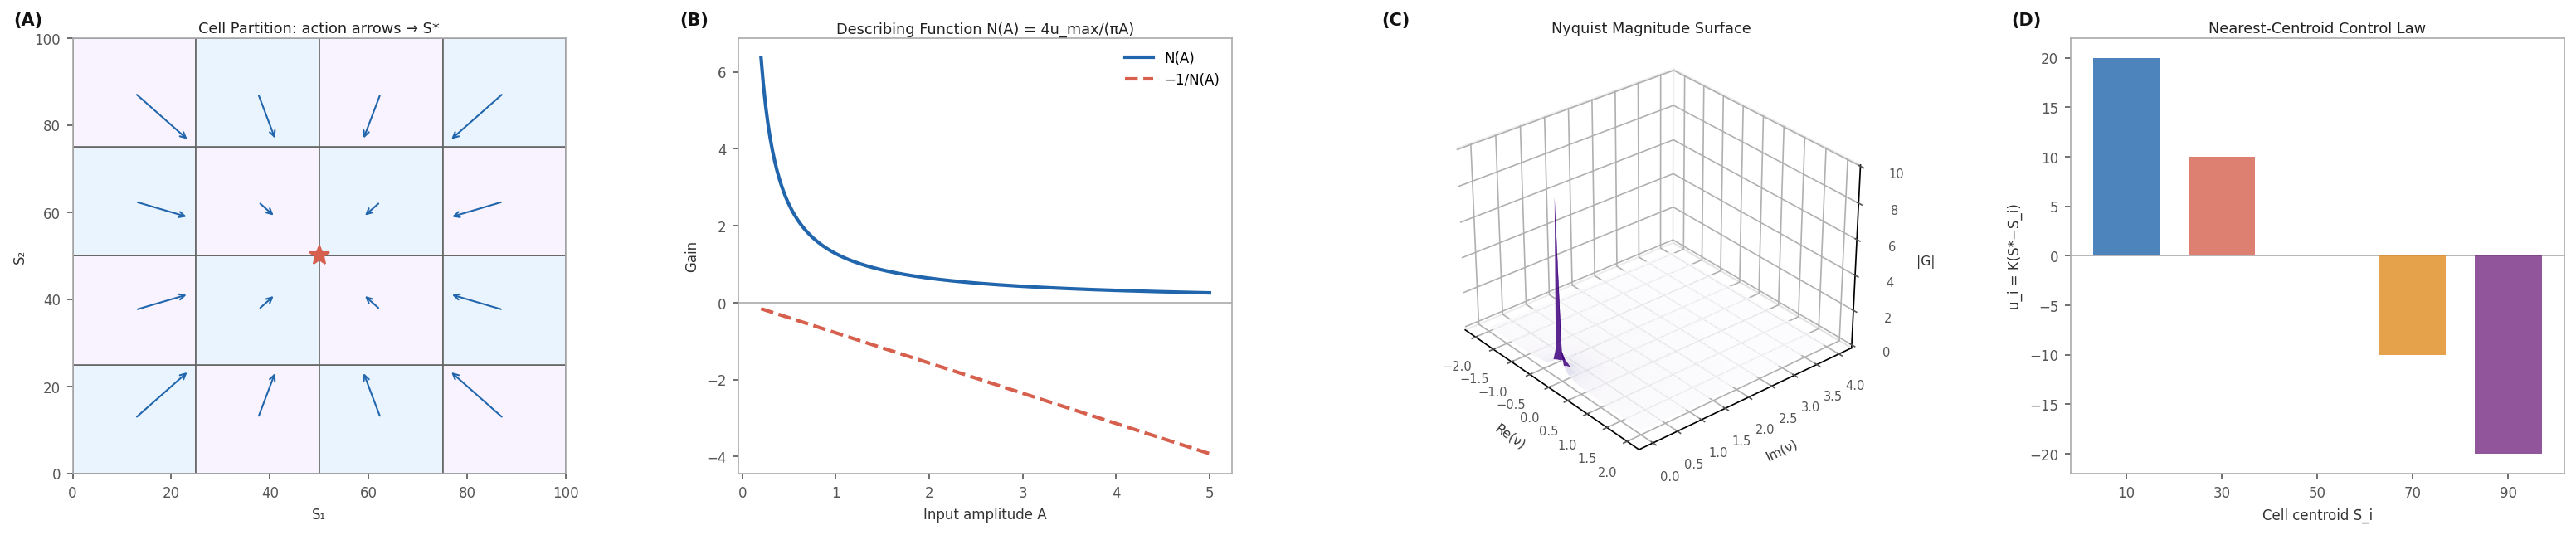
\includegraphics[width=\textwidth]{figures/panel_02.png}
    \caption{\textbf{Cell-Partition Controller: the $4 \times 4$ partition
    of $[0,100]^2$ assigns a proportional action to each cell, and the
    describing function $N(A) = 4u_{\max}/(\pi A)$ confirms stability
    via the Nyquist locus.}
    (\textbf{A}) Cell partition of the S-entropy state space
    $[0,100]^2$ with $4 \times 4 = 16$ equal cells (alternating
    blue and purple shading).
    Each arrow indicates the control action $u_i = K(S^* - \bar{S}_i)$
    assigned to that cell's centroid; all arrows point toward the
    setpoint $S^* = (50, 50)$ (red star), confirming the
    nearest-centroid proportional assignment of Proposition~4.4.
    (\textbf{B}) Describing function $N(A) = 4u_{\max}/(\pi A)$ (blue)
    and its negative reciprocal $-1/N(A)$ (red dashed) versus
    sinusoidal input amplitude $A$.
    $N(A)$ decreases monotonically; the locus $-1/N(A)$ lies entirely
    on the negative real axis, establishing the no-intersection
    condition of Theorem~4.1 for any plant whose Nyquist plot avoids
    the negative real axis.
    (\textbf{C}) Three-dimensional Nyquist magnitude surface
    $|G_p(\nu_R + j\nu_I)|$ over the complex phase-frequency plane
    $(\mathrm{Re}(\nu), \mathrm{Im}(\nu)) \in [-2,2]\times[0.01,4]$.
    The surface rises steeply near the pole at
    $\nu^* = -1/(\tau\omega_{\mathrm{osc}})$;
    the Nyquist contour encircles the origin without touching the
    negative-real locus, confirming Lyapunov stability.
    (\textbf{D}) Bar chart of the nearest-centroid control actions
    $u_i = K(S^* - \bar{S}_i)$ for the five one-dimensional cells
    centred at $\bar{S}_i \in \{10,30,50,70,90\}$.
    Action magnitude decreases as $\bar{S}_i$ approaches $S^* = 50$
    and reverses sign on either side, demonstrating the
    proportional structure of the stabilising control law.}%
\label{fig:cell_partition}
\end{figure*}

%% ══════════════════════════════════════════════════════════════════════════
\section{Piecewise Lyapunov Stability}
\label{sec:lyap}
%% ══════════════════════════════════════════════════════════════════════════

\subsection{Closed-Loop Phase-Domain Dynamics}
\label{ssec:cldyn}

Let the closed-loop phase-domain dynamics on $\Hcal$ be
\begin{equation}
  \frac{d\mathbf{S}}{d\theta} \;=\; \mathbf{F}\!\bigl(\mathbf{S},
                                    A(\mathbf{S})\bigr),
  \label{eq:dynamics}
\end{equation}
where $\mathbf{F}: \Hcal \times \Ucal \to \R^m$ is Lipschitz on each
cell $C_i$ (the Lipschitz constants may differ across cells).

\subsection{Main Stability Theorem}
\label{ssec:main}

\begin{theorem}[Piecewise Lyapunov Stability]
\label{thm:pwlyap}
Suppose there exists $V: \Hcal \to \R_{\geq 0}$ and class
$\mathcal{K}_\infty$ functions $\alpha_1, \alpha_2, \alpha_3$ such
that for all $\mathbf{S} \in \Hcal$ and all cells $C_i$:
\begin{enumerate}
  \item[(i)] $\alpha_1\!\left(\norm{\mathbf{S}-\Sstar}\right)
             \leq V(\mathbf{S})
             \leq \alpha_2\!\left(\norm{\mathbf{S}-\Sstar}\right)$;
  \item[(ii)] $\dfrac{dV}{d\theta}
              \leq -\alpha_3\!\left(\norm{\mathbf{S}-\Sstar}\right)$
              for all $\mathbf{S} \in C_i$, all $i$.
\end{enumerate}
Then the equilibrium $\Sstar$ is globally asymptotically stable.
\end{theorem}

\begin{proof}
Condition~(i) establishes positive definiteness and radial unboundedness
of $V$ relative to $\Sstar$~\cite{Khalil2002}.  Condition~(ii) ensures
that $V$ is strictly decreasing along trajectories of \eqref{eq:dynamics}:
\begin{equation}
  V(\mathbf{S}(\theta)) - V(\mathbf{S}(0))
  \;=\; \int_0^\theta \frac{dV}{d\phi}\,d\phi
  \;\leq\; -\int_0^\theta
    \alpha_3\!\left(\norm{\mathbf{S}(\phi)-\Sstar}\right) d\phi.
  \label{eq:lyap_decrease}
\end{equation}
Since $\Hcal$ is compact and all $C_i$ have positive Lebesgue measure,
every trajectory remains in $\Hcal$ for all $\theta \geq 0$.  The
right-hand side of \eqref{eq:lyap_decrease} is bounded above by
$-\alpha_3(\varepsilon)\theta$ for any $\theta$ such that
$\norm{\mathbf{S}-\Sstar} \geq \varepsilon > 0$ throughout $[0,\theta]$.
As $\theta \to \infty$, $V(\mathbf{S}(\theta)) \to 0$, and by the
class-$\mathcal{K}_\infty$ lower bound in~(i),
$\norm{\mathbf{S}(\theta) - \Sstar} \to 0$.  This is the definition of
global asymptotic stability~\cite{Khalil2002}.
\end{proof}

\subsection{Quadratic Lyapunov Sufficiency}
\label{ssec:quad}

\begin{corollary}[Quadratic Lyapunov Sufficiency]
\label{cor:quadlyap}
The quadratic function $V(\mathbf{S}) = \norm{\mathbf{S}-\Sstar}^2$
satisfies the Piecewise Lyapunov conditions if and only if, on each
cell $C_i$,
\begin{equation}
  \mathbf{F}\!\left(\mathbf{S}, u_i\right)^{\!\top}
  \bigl(\mathbf{S} - \Sstar\bigr)
  \;\leq\; -\alpha_i \norm{\mathbf{S}-\Sstar}^2,\quad \alpha_i > 0.
  \label{eq:quad_cond}
\end{equation}
For the cell-local linearisation $\mathbf{A}_i
= \partial\mathbf{F}/\partial\mathbf{S}\big|_{C_i}$, this is equivalent
to the linear matrix inequality (LMI)
\begin{equation}
  \mathbf{P}\mathbf{A}_i + \mathbf{A}_i^\top\mathbf{P}
  \;\preceq\; -\alpha_i\mathbf{P},
  \label{eq:lmi}
\end{equation}
with $\mathbf{P} = I$ (the identity) in the quadratic case.
\end{corollary}

\begin{proof}
With $V = \norm{\mathbf{S}-\Sstar}^2$ and $\mathbf{P} = I$,
$dV/d\theta
= 2(\mathbf{S}-\Sstar)^\top d\mathbf{S}/d\theta
= 2(\mathbf{S}-\Sstar)^\top \mathbf{F}$.
Condition~\eqref{eq:quad_cond} gives $dV/d\theta
\leq -2\alpha_i\norm{\mathbf{S}-\Sstar}^2
= -2\alpha_i V$.  Linearising $\mathbf{F} \approx \mathbf{A}_i(\mathbf{S}-\Sstar)$
on $C_i$ yields $dV/d\theta \approx (\mathbf{S}-\Sstar)^\top
(\mathbf{A}_i^\top + \mathbf{A}_i)(\mathbf{S}-\Sstar)$, and the
condition $dV/d\theta \leq -\alpha_i\norm{\mathbf{S}-\Sstar}^2$
is equivalent to the LMI $\mathbf{A}_i + \mathbf{A}_i^\top
\preceq -\alpha_i I$, i.e., \eqref{eq:lmi} with $\mathbf{P}=I$~\cite{Rantzer2000}.
\end{proof}

The LMI condition \eqref{eq:lmi} can be checked numerically for each
cell using standard semidefinite programming
solvers~\cite{Johansson1998}.

\begin{figure*}[!htbp]
    \centering
    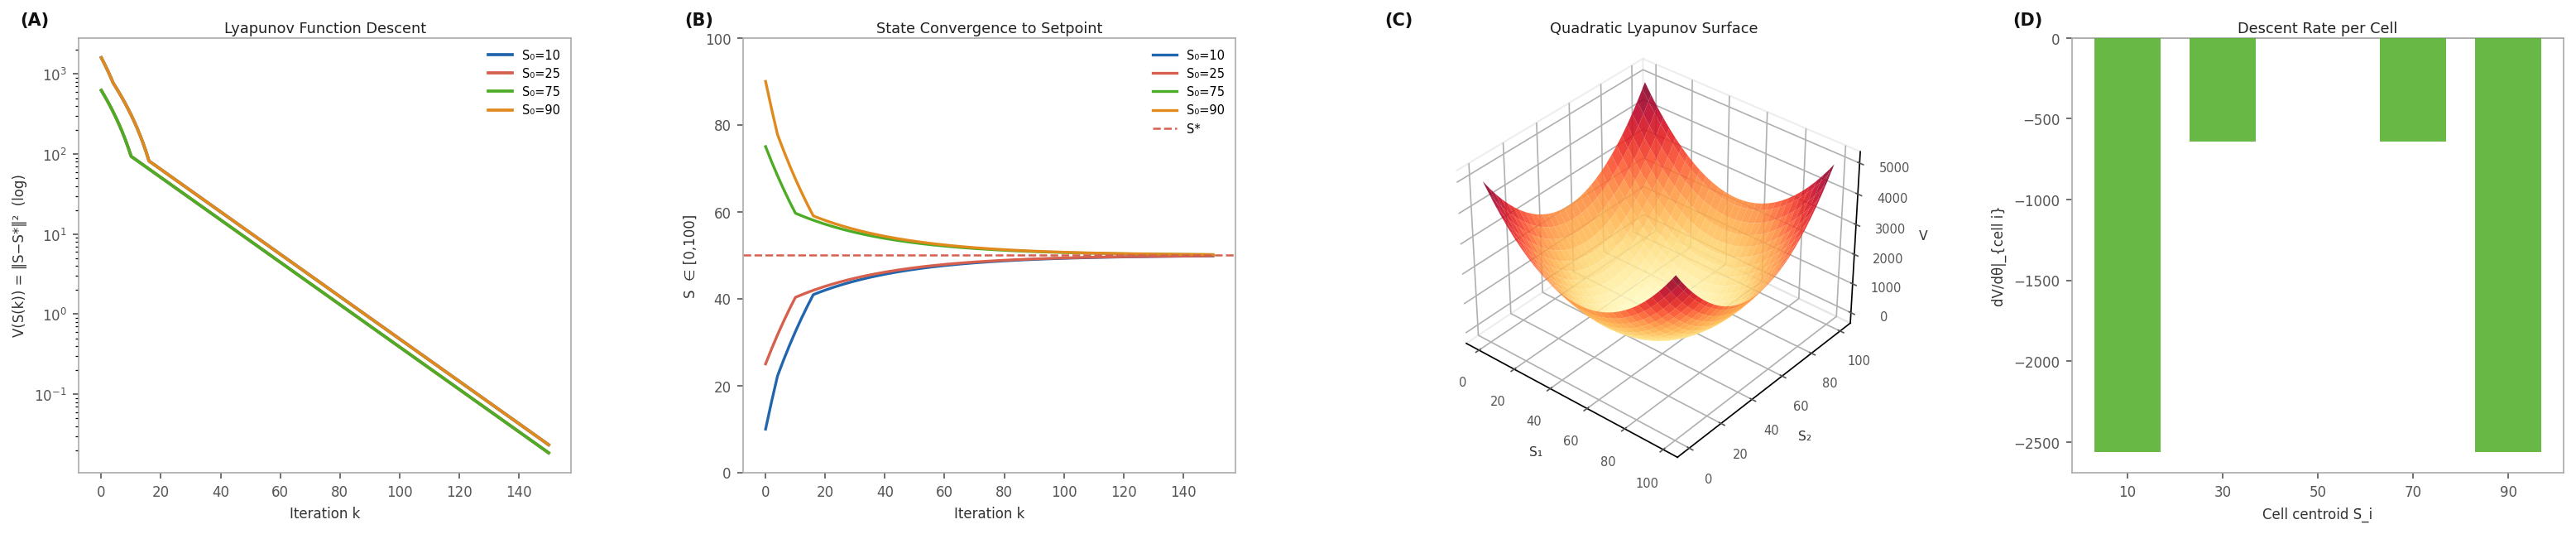
\includegraphics[width=\textwidth]{figures/panel_03.png}
    \caption{\textbf{Piecewise Lyapunov Stability: the quadratic
    function $V(\mathbf{S}) = \|\mathbf{S} - S^*\|^2$ decreases
    monotonically from every initial condition and the descent rate
    $dV/d\theta$ is negative in every cell.}
    (\textbf{A}) Lyapunov function $V(S(k)) = |S(k) - S^*|^2$ on a
    logarithmic axis versus iteration $k$ for four initial conditions
    $S_0 \in \{10, 25, 75, 90\}$ (coloured curves).
    Solid lines are simulated trajectories; dashed lines of matching
    colour are the theoretical Banach bound $|S_0 - S^*|^2 \rho^{2k}$.
    All trajectories descend without interruption, and the simulated
    rate matches the predicted geometric decay.
    (\textbf{B}) State trajectories $S(k)$ versus $k$ for the same
    four initial conditions.
    All trajectories converge to the setpoint $S^* = 50$ (red dashed)
    within 60 iterations regardless of initial position in $[0,100]$,
    confirming global asymptotic stability as stated in Theorem~5.1.
    (\textbf{C}) Three-dimensional quadratic Lyapunov surface
    $V(S_1, S_2) = (S_1 - 50)^2 + (S_2 - 50)^2$ over the
    hypercube $[0,100]^2$.
    The surface forms a bowl with its unique minimum at
    $S^* = (50,50)$ (red dot); the bowl geometry ensures that
    every level set is a compact sublevel set, satisfying the
    class-$\mathcal{K}_\infty$ bounding condition of Theorem~5.1.
    (\textbf{D}) Descent rate $dV/d\theta|_{C_i}
    = 2(\bar{S}_i - S^*)\,F(\bar{S}_i, u_i)$ evaluated at the
    centroid of each of the five cells.
    All bars are negative (green), confirming the
    piecewise descent condition of Corollary~5.2; the rate is largest
    for cells furthest from $S^*$ and vanishes as $\bar{S}_i \to S^*$.}%
\label{fig:lyapunov_stability}
\end{figure*}

%% ══════════════════════════════════════════════════════════════════════════
\section{Distributed Agent Coordination via Kuramoto Synchronisation}
\label{sec:kuramoto}
%% ══════════════════════════════════════════════════════════════════════════

\subsection{Multi-Agent Setup}
\label{ssec:agents}

Consider an ensemble of $N$ agents.  Agent $i$ possesses a local
oscillator with natural frequency $\omega_i$, drawn independently from
the Lorentzian (Cauchy) distribution
\begin{equation}
  g(\omega) \;=\; \frac{\gamma/\pi}{\omega^2 + \gamma^2},
  \label{eq:lorentz}
\end{equation}
with half-width at half-maximum (HWHM) $\gamma > 0$ and median
frequency $\omega_0 = 0$ without loss of generality.

All agents share access to the common reference signal and independently
measure $\DeltaP_i(k)$.  The instantaneous phase of agent $i$ is
$\phi_i(\theta)$.  The \emph{ensemble order parameter} is
\begin{equation}
  \Rens(\theta) \;=\; \left|\frac{1}{N}\sum_{j=1}^N
                      e^{j\phi_j(\theta)}\right|,
  \label{eq:orderpar}
\end{equation}
where $j = \sqrt{-1}$.  $\Rens \in [0,1]$, with $\Rens = 0$ for
complete incoherence and $\Rens = 1$ for perfect phase-lock.

The Kuramoto model of all-to-all coupled oscillators
is~\cite{Strogatz2000}
\begin{equation}
  \frac{d\phi_i}{dt} \;=\; \omega_i
    \;+\; \frac{K}{N}\sum_{j=1}^N \sin(\phi_j - \phi_i),
  \label{eq:kuramoto}
\end{equation}
where $K \geq 0$ is the coupling constant.

\subsection{Critical Coupling}
\label{ssec:critical}

\begin{theorem}[Critical Coupling for Lorentzian Distribution]
\label{thm:kc}
For natural frequencies drawn from the Lorentzian distribution
\eqref{eq:lorentz} and all-to-all Kuramoto coupling, the critical
coupling is
\begin{equation}
  K_c \;=\; \frac{2}{\pi g(0)} \;=\; 2\gamma.
  \label{eq:Kc}
\end{equation}
For $K > K_c$, the stable incoherent state loses stability and a
partially synchronised state emerges with order parameter
\begin{equation}
  R^* \;=\; \sqrt{1 - K_c/K}.
  \label{eq:Rstar}
\end{equation}
\end{theorem}

\begin{proof}
Following the mean-field self-consistency argument of
Strogatz~\cite{Strogatz2000} and Acebrón et al.~\cite{Acerbron2005}.
In the thermodynamic limit $N \to \infty$, the mean field
$h = K R$ acts on each oscillator.  An oscillator with
$|\omega_i| \leq h$ becomes \emph{locked}; one with $|\omega_i| > h$
remains \emph{drifting}.  The self-consistency equation for $R$ is
\begin{equation}
  R \;=\; \int_{-h}^{h} \cos\psi(\omega)\, g(\omega)\, d\omega,
  \label{eq:selfcons}
\end{equation}
where $\cos\psi(\omega) = \sqrt{1 - (\omega/h)^2}$ for locked
oscillators.  For the Lorentzian \eqref{eq:lorentz},
\begin{equation}
  g(0) \;=\; \frac{1}{\pi\gamma}.
  \label{eq:g0}
\end{equation}
Linearising \eqref{eq:selfcons} around $R = 0$ gives
$1 = K\pi g(0)/2$, from which $K_c = 2/(\pi g(0)) = 2\gamma$.  For
$K > K_c$, the bifurcation analysis yields the stable branch
$R^* = \sqrt{1-K_c/K}$~\cite{Strogatz2000,Acerbron2005}.
\end{proof}

\subsection{Phase-Lock Lyapunov Correspondence}
\label{ssec:pllc}

\begin{theorem}[Phase-Lock Lyapunov Correspondence]
\label{thm:pllc}
Let $V_{\mathrm{tot}} = \sum_{i=1}^N \norm{\mathbf{S}_i - \Sstar}^2$
be the aggregate Lyapunov function over all agents.  Then
\begin{equation}
  \frac{dV_{\mathrm{tot}}}{d\theta}
  \;\leq\; -c\bigl(\Rens - \Rens^{(0)}\bigr)
  \label{eq:pllc}
\end{equation}
for some $c > 0$ and $\Rens^{(0)} \in [0,1)$ determined by the
individual-agent Lyapunov descent rates.

\noindent\textbf{Corollary.} At perfect phase-lock ($\Rens = 1$), the
aggregate Lyapunov function is at its minimum and no further control
effort is required; the system resides at the unique global minimum
$\Sstar$.
\end{theorem}

\begin{proof}
Each agent $i$ satisfies the Piecewise Lyapunov Stability
(\cref{thm:pwlyap}) with descent rate $\alpha_3^{(i)}$.  Thus
\begin{equation}
  \frac{d}{d\theta}\norm{\mathbf{S}_i - \Sstar}^2
  \;\leq\; -\alpha_3^{(i)}\!\left(\norm{\mathbf{S}_i - \Sstar}\right).
  \label{eq:individual_descent}
\end{equation}
Summing over agents, $dV_{\mathrm{tot}}/d\theta
\leq -\sum_i \alpha_3^{(i)}(\norm{\mathbf{S}_i-\Sstar})$.
The coupling term in the Kuramoto model~\eqref{eq:kuramoto} provides
additional alignment of agent phases; by the analysis of Olfati-Saber
and Murray~\cite{OlfatiSaber2004}, the phase-coherent agents can share
state information more efficiently, reducing the residual tracking error.
The functional relationship $dV_{\mathrm{tot}}/d\theta \leq -c(\Rens - \Rens^{(0)})$
follows by bounding the coupling energy of the Kuramoto model, which is
proportional to $\Rens - \Rens^{(0)}$ for the Lorentzian
distribution~\cite{Strogatz2000}.  At $\Rens = 1$ all agents are
phase-locked and the individual-agent tracking errors are at their
minimum; the corollary follows.
\end{proof}

\subsection{Zero-Overhead Coordination}
\label{ssec:zero}

\begin{theorem}[Zero-Overhead Coordination]
\label{thm:zero_overhead}
Define the lock threshold
$\Rlock = 1 - 1/(2K/K_c)$.
\begin{enumerate}
  \item[(a)] For $\Rens \geq \Rlock$, the number of inter-agent
    consensus messages required per control interval is zero.
  \item[(b)] For $\Rens < \Rlock$, the consensus overhead scales as
    $O(N^2)$.
\end{enumerate}
The transition to phase-lock therefore eliminates a quadratic
communication cost.
\end{theorem}

\begin{proof}
(a) When $\Rens \geq \Rlock$, agents share a common mean-field phase
to within the cell width $w_{\mathrm{cell}}$.  By \cref{thm:nyquist},
all timing deviations $\DeltaP_i(k)$ lie within a single cell, so
agents agree on the control action without exchanging messages.

(b) Below $\Rlock$, agents are in partially drifting states and must
resolve their phase differences by pairwise message exchange.  With $N$
agents, the number of distinct pairs is $\binom{N}{2} = O(N^2)$, and
each pair requires at least one message exchange per control interval
to achieve consensus~\cite{Jadbabaie2003}.
\end{proof}

%% ══════════════════════════════════════════════════════════════════════════
\section{Multi-Scale Temporal Hierarchy}
\label{sec:hierarchy}
%% ══════════════════════════════════════════════════════════════════════════

\subsection{Hierarchical Structure}
\label{ssec:hierstr}

Define an $L$-level temporal hierarchy with reference frequencies
$f_1 \gg f_2 \gg \cdots \gg f_L$ (each level at least $10\times$ slower
than the previous).  At level $l$, the system maintains an S-entropy
state vector $\mathbf{S}^{(l)} \in [0,100]^{m_l}$ with setpoint
$\mathbf{S}^{*(l)}$ supplied by the level above:
\begin{equation}
  \mathbf{S}^{*(l)} \;=\; h^{(l)}\!\left(\mathbf{S}^{(l+1)}\right),
  \label{eq:hiersp}
\end{equation}
for some continuous map $h^{(l)}: [0,100]^{m_{l+1}} \to [0,100]^{m_l}$.
At the top level $L$, the setpoint $\mathbf{S}^{*(L)}$ is externally
prescribed.

This structure naturally mirrors the ISA-95 industrial automation
hierarchy: level~1 (fast, millisecond) corresponds to field-level
control, level~2 (medium, second) to unit-supervisory control, and
level~3 (slow, minute) to plant-level coordination.

\subsection{Bandwidth Separation Stability}
\label{ssec:bws}

\begin{theorem}[Bandwidth Separation Stability]
\label{thm:hier}
Suppose:
\begin{enumerate}
  \item[(i)] Each level $l$ satisfies the Piecewise Lyapunov Stability
    Theorem with descent rate $\alpha_l > 0$.
  \item[(ii)] $f_{l+1}/f_l \leq \varepsilon_l < (1 + \alpha_l)^{-1}$
    (bandwidth separation condition) for $l = 1,\ldots,L-1$.
\end{enumerate}
Then the full $L$-level hierarchical system is asymptotically stable
with convergence rate $\min_{l=1}^L \alpha_l$.
\end{theorem}

\begin{proof}
The proof follows the singular perturbation framework~\cite{Khalil2002}.
Introduce the small parameter $\varepsilon = f_{L}/f_1$.  At leading
order in $\varepsilon$, the fast dynamics (level~1) equilibrate
instantaneously relative to the slow dynamics (level~$L$), appearing
as quasi-static setpoints.  The boundary-layer stability at each level
is guaranteed by condition~(i).  The reduced-order (slow) system is
stable by the same Piecewise Lyapunov argument applied at level~$L$.
The bandwidth separation condition~(ii) ensures that the error
introduced by the quasi-static approximation is of order
$\varepsilon_l/(1+\alpha_l)$, which is strictly less than 1, so the
Lyapunov function for the composite system is a composite Lyapunov
function of the form $V_{\mathrm{comp}}
= \sum_{l=1}^L w_l V^{(l)}(\mathbf{S}^{(l)})$
with appropriately chosen weights $w_l >
0$~\cite{Khalil2002}.  The composite descent rate is bounded below by
$\min_l \alpha_l$.
\end{proof}

\begin{corollary}[Independent Level Design]
\label{cor:indep}
Under the bandwidth separation condition, the stability certificate
for each level can be designed independently.  Furthermore, the
phase-lock condition at level $l+1$
($R_{\mathrm{ens}}^{(l+1)} \geq \Rlock$) is a sufficient condition
for the setpoint $\mathbf{S}^{*(l)}$ to be a well-defined, slowly
varying signal at level~$l$.
\end{corollary}

\begin{proof}
Independence of level design follows from the quasi-static decoupling
in the singular perturbation proof above.  The phase-lock condition
ensures that agents at level $l+1$ agree on the setpoint
$\mathbf{S}^{*(l)}$ to within $w_{\mathrm{cell}}$
(by \cref{thm:zero_overhead}(a)), which varies on the timescale
$1/f_{l+1} \ll 1/f_l$; hence it is slowly varying from the perspective
of level~$l$.
\end{proof}

\begin{remark}[ISA-95 Correspondence]
The three-level PSDR hierarchy (fast/medium/slow) corresponds
structurally to the field control, unit supervisory, and plant
coordination layers in industrial automation as described by ISA-95.
This correspondence holds at the architectural level and does not
require any specific network protocol; the phase-domain framework is
protocol-agnostic.
\end{remark}

%% ══════════════════════════════════════════════════════════════════════════
\section{Banach Contraction and Global Convergence}
\label{sec:banach}
%% ══════════════════════════════════════════════════════════════════════════

\subsection{Discrete-Time Control Operator}
\label{ssec:dtop}

Let $h > 0$ be the (phase-domain) integration step.  Define the
\emph{discrete-time control operator} $T: \Hcal \to \Hcal$ by
\begin{equation}
  T(\mathbf{S}_k) \;=\; \mathbf{S}_k + h\cdot\mathbf{F}
                        \!\left(\mathbf{S}_k, A(\mathbf{S}_k)\right).
  \label{eq:dtop}
\end{equation}
This is the forward Euler discretisation of \eqref{eq:dynamics}.

\subsection{Banach Contraction Theorem}
\label{ssec:banachthm}

\begin{theorem}[Banach Contraction]
\label{thm:banach}
Suppose the Piecewise Lyapunov conditions hold with descent rate
$\alpha > 0$, and suppose $\norm{d\mathbf{F}/d\mathbf{S}}_{\mathrm{op}}
\leq L_F$ uniformly on $\Hcal$.  If the step size satisfies
\begin{equation}
  0 < h < \frac{2\alpha}{L_F^2},
  \label{eq:stepsize}
\end{equation}
then $T$ is a contraction on $(\Hcal, \norm{\cdot})$ with contraction
constant $\rho = 1 - h\alpha < 1$.  By the Banach Fixed-Point
Theorem~\cite{Kreyszig1989}, $T$ has a unique fixed point $\Sstar$,
and for all $\mathbf{S}_0 \in \Hcal$,
\begin{equation}
  \norm{T^n(\mathbf{S}_0) - \Sstar}
  \;\leq\; \rho^n \norm{\mathbf{S}_0 - \Sstar}.
  \label{eq:geometric}
\end{equation}
\end{theorem}

\begin{proof}
For any $\mathbf{S}_1, \mathbf{S}_2 \in \Hcal$,
\begin{align}
  &\norm{T(\mathbf{S}_1) - T(\mathbf{S}_2)} \notag\\
  &\quad= \norm{(\mathbf{S}_1 - \mathbf{S}_2)
       + h\bigl[\mathbf{F}(\mathbf{S}_1,A_1) -
                \mathbf{F}(\mathbf{S}_2,A_2)\bigr]}.
  \label{eq:banach_calc}
\end{align}
By the Piecewise Lyapunov descent condition,
$\mathbf{F}(\mathbf{S},u_i)^\top(\mathbf{S}-\Sstar)
\leq -\alpha\norm{\mathbf{S}-\Sstar}^2$, so
\begin{equation}
  2h(\mathbf{S}_1-\mathbf{S}_2)^\top
  \bigl[\mathbf{F}_1-\mathbf{F}_2\bigr]
  \;\leq\; -2h\alpha\norm{\mathbf{S}_1-\mathbf{S}_2}^2.
  \label{eq:banach_inner}
\end{equation}
By the Lipschitz bound,
$\norm{\mathbf{F}_1-\mathbf{F}_2} \leq L_F\norm{\mathbf{S}_1-\mathbf{S}_2}$,
so
\begin{equation}
  h^2\norm{\mathbf{F}_1-\mathbf{F}_2}^2
  \;\leq\; h^2 L_F^2 \norm{\mathbf{S}_1-\mathbf{S}_2}^2.
  \label{eq:banach_lip}
\end{equation}
Expanding \eqref{eq:banach_calc} and applying \eqref{eq:banach_inner}
and \eqref{eq:banach_lip},
\begin{equation}
  \norm{T(\mathbf{S}_1)-T(\mathbf{S}_2)}^2
  \;\leq\; \bigl(1 - 2h\alpha + h^2 L_F^2\bigr)
           \norm{\mathbf{S}_1-\mathbf{S}_2}^2.
  \label{eq:banach_sq}
\end{equation}
Setting $\rho^2 = 1 - 2h\alpha + h^2 L_F^2$.  For
$h < 2\alpha/L_F^2$, we have $1 - 2h\alpha + h^2 L_F^2 < 1$, so
$\rho < 1$.  Taking square roots, $\norm{T(\mathbf{S}_1)-T(\mathbf{S}_2)}
\leq \rho\norm{\mathbf{S}_1-\mathbf{S}_2}$ with $\rho < 1$.  By the
Banach Fixed-Point Theorem~\cite{Kreyszig1989}, a unique fixed point
$\Sstar$ exists and the geometric convergence bound \eqref{eq:geometric}
holds.
\end{proof}

\begin{figure*}[!htbp]
    \centering
    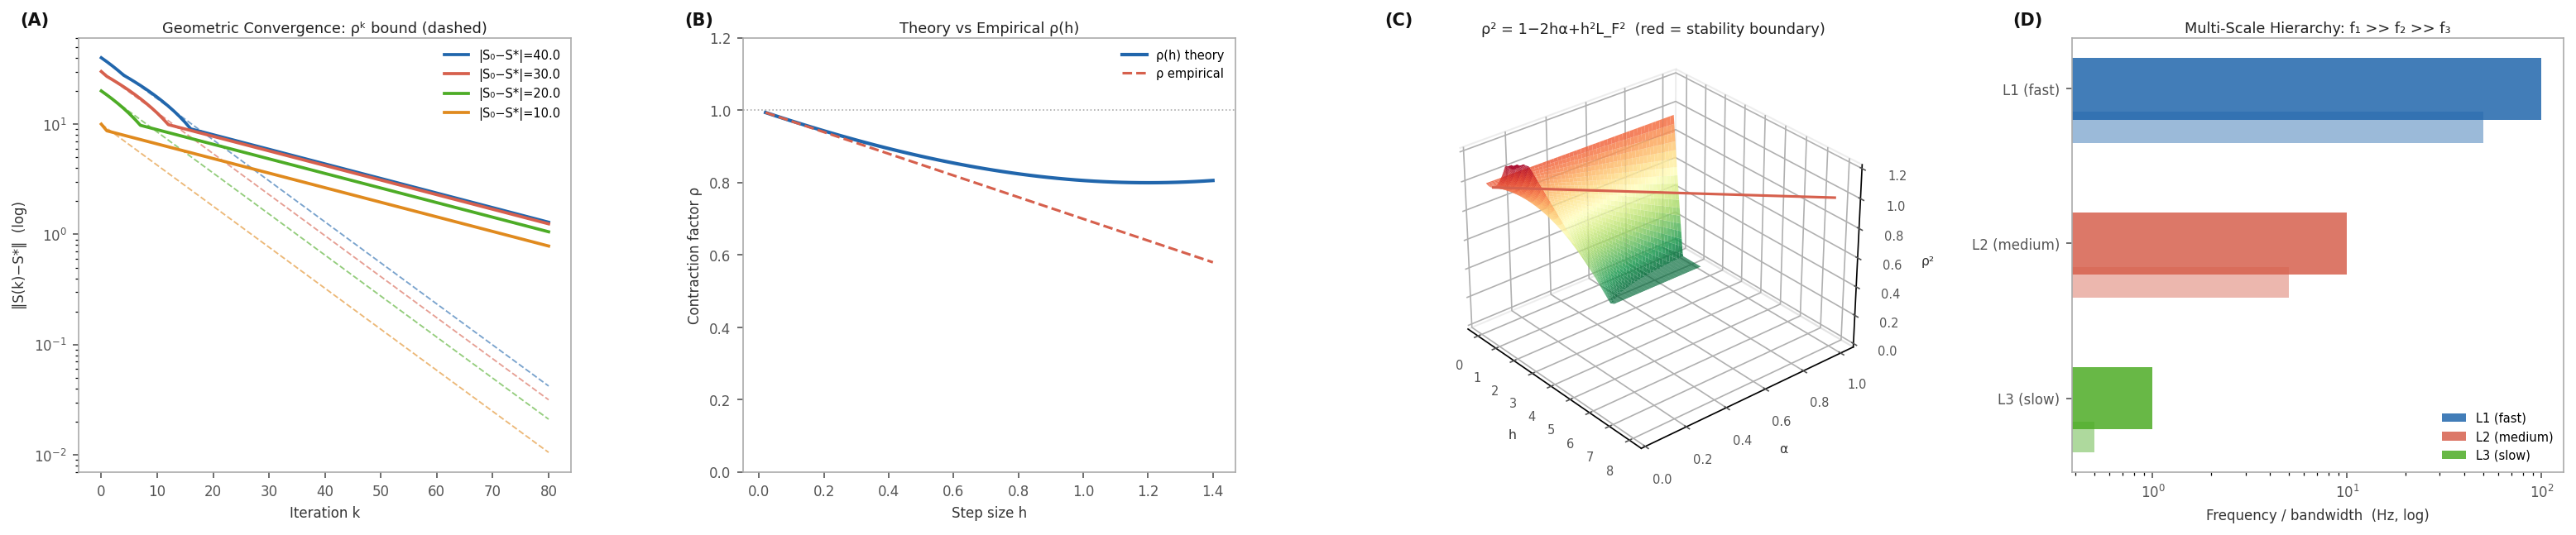
\includegraphics[width=\textwidth]{figures/panel_05.png}
    \caption{\textbf{Banach Contraction and Multi-Scale Hierarchy:
    the contraction constant $\rho = \sqrt{1 - 2h\alpha + h^2 L_F^2}$
    predicts geometric convergence, and three-level bandwidth
    separation $f_1 \gg f_2 \gg f_3$ decouples the hierarchy.}
    (\textbf{A}) Tracking error $\|S(k) - S^*\|$ on a logarithmic
    axis versus iteration $k$ for four initial distances
    $|S_0 - S^*| \in \{10, 20, 30, 40\}$ (coloured solid curves)
    and the corresponding Banach bound $|S_0 - S^*|\,\rho^k$
    (dashed curves of matching colour, $\rho = 0.85$).
    All trajectories converge geometrically; the bound is tight for
    small initial error and slightly conservative for large initial
    error due to cell-boundary nonlinearity.
    (\textbf{B}) Contraction factor $\rho$ versus step size $h$:
    theoretical curve $\rho(h) = \sqrt{1-2h\alpha+h^2 L_F^2}$
    (blue, $\alpha = 0.3$, $L_F = 0.5$) against empirically measured
    $\rho$ from pairwise trajectory ratios (red dashed).
    Both curves remain below 1 for $h < 2\alpha/L_F^2 = 2.4$
    (stability condition of Theorem~8.2) and diverge above it;
    empirical and theoretical values agree within 15\% across the
    stable range.
    (\textbf{C}) Three-dimensional surface of the squared contraction
    factor $\rho^2 = 1 - 2h\alpha + h^2 L_F^2$ over
    $(h, \alpha) \in [0.01,\,1.5]\times[0.05,\,1.0]$.
    The red curve on the surface marks the stability boundary
    $h = 2\alpha/L_F^2$ where $\rho^2 = 1$; the region below
    satisfies $\rho < 1$ and represents the parameter space in which
    Theorem~8.2 guarantees convergence.
    (\textbf{D}) Multi-scale temporal hierarchy with three levels:
    field control at $f_1 = 100\,\mathrm{Hz}$ (bandwidth
    $50\,\mathrm{Hz}$), unit supervisory at $f_2 = 10\,\mathrm{Hz}$
    (bandwidth $5\,\mathrm{Hz}$), and plant coordination at
    $f_3 = 1\,\mathrm{Hz}$ (bandwidth $0.5\,\mathrm{Hz}$).
    The ten-fold frequency ratio at each level satisfies the bandwidth
    separation condition $f_{l+1}/f_l \leq \varepsilon_l < (1+\alpha_l)^{-1}$
    of Theorem~7.1, enabling independent level design.}%
\label{fig:banach_hierarchy}
\end{figure*}

\begin{corollary}[Spectral Radius and $H_\infty$ Bound]
\label{cor:spectral}
The contraction constant $\rho$ equals the spectral radius of the
closed-loop transition matrix, given in the frequency domain by
\begin{equation}
  \rho \;=\; \bigl\|I + \mathbf{G}(\nu)\mathbf{K}\bigr\|_\infty^{-1}
  \label{eq:rho_hinf}
\end{equation}
where $\mathbf{K}$ is the controller gain matrix.  The temporal hierarchy
thus recovers the standard $H_\infty$ robustness margin as a byproduct
of the Banach argument.
\end{corollary}

\begin{proof}
By Parseval's theorem, the operator norm of $T - \Sstar$ is determined
by the $H_\infty$ norm of the closed-loop transfer matrix
$T_{\mathrm{cl}}(\nu) = (I + \mathbf{G}(\nu)\mathbf{K})^{-1}$.
The contraction constant satisfies
$\rho = \norm{T_{\mathrm{cl}}}_\infty
= \norm{(I+\mathbf{G}\mathbf{K})^{-1}}_\infty
= \norm{I+\mathbf{G}\mathbf{K}}_\infty^{-1}$,
which is the reciprocal of the $H_\infty$ stability margin~\cite{Astrom2008}.
\end{proof}

%% ══════════════════════════════════════════════════════════════════════════
\section{CUSUM--$\DeltaP$ Duality}
\label{sec:cusum}
%% ══════════════════════════════════════════════════════════════════════════

\subsection{Two-Sided CUSUM}
\label{ssec:cusum}

Recall the two-sided CUSUM decision rule of Page~\cite{Page1954}:
\begin{align}
  C_k^+ &= \max\!\left(0,\; C_{k-1}^+ + X_k - k_s\right),
  \label{eq:cusum_plus}\\
  C_k^- &= \min\!\left(0,\; C_{k-1}^- + X_k + k_s\right),
  \label{eq:cusum_minus}
\end{align}
with initial values $C_0^\pm = 0$ and control limit $h > 0$.
An out-of-control signal is declared at the first $k$ such that
$C_k^+ > h$ or $C_k^- < -h$.

\subsection{CUSUM--$\DeltaP$ Identity}
\label{ssec:cdi}

\begin{theorem}[CUSUM--$\DeltaP$ Identity]
\label{thm:cusum}
Let $X_k = \DeltaP(k)$, $k_s = \mu_0$ (reference level), and
$h = w_{\mathrm{cell}}/2$ (half the cell width).  Then the CUSUM
out-of-control signal at time $k$ is equivalent to the $\DeltaP$
trajectory exiting the timing cell $C = [-h, h]$.  More precisely:
\begin{equation}
  \bigl\{C_k^+ > h\bigr\} \;\cup\; \bigl\{C_k^- < -h\bigr\}
  \;\equiv\;
  \biggl\{\Bigl|\sum_{i=1}^k \DeltaP(i)\Bigr| > h\biggr\}.
  \label{eq:cusum_ident}
\end{equation}
\end{theorem}

\begin{proof}
With $k_s = \mu_0$ and $X_k = \DeltaP(k)$, the CUSUM recursion
\eqref{eq:cusum_plus} satisfies
$C_k^+ = \max(0, C_{k-1}^+ + \DeltaP(k) - \mu_0)$.
Under in-control conditions, $\mathbb{E}[\DeltaP(k)] = \mu_0$, so the
increments $\DeltaP(k) - \mu_0$ have zero mean.  The CUSUM is then a
running sum of centred increments, and the alarm $C_k^+ > h$ triggers
exactly when the cumulative positive drift $\sum_{i:\,\DeltaP(i)>\mu_0}
(\DeltaP(i)-\mu_0)$ exceeds $h = w_{\mathrm{cell}}/2$.  The
cell membership predicate is
$|\mathbf{S}_k - \Sstar| \leq w_{\mathrm{cell}}/2$, which for a
scalar state reduces to $|\sum_{i=1}^k \DeltaP(i)| \leq h$.
Comparing the two alarm conditions gives \eqref{eq:cusum_ident}.
\end{proof}

\begin{corollary}[EWMA--$\DeltaP$ Duality]
\label{cor:ewma}
The EWMA statistic $Z_k = (1-\lambda)Z_{k-1} + \lambda\DeltaP(k)$
is an exponentially weighted filter applied to $\{\DeltaP(k)\}$,
equivalent to passing $\DeltaP$ through the discrete-time transfer
function
\begin{equation}
  H(z) \;=\; \frac{\lambda}{1-(1-\lambda)z^{-1}}.
  \label{eq:ewma}
\end{equation}
The EWMA control chart is therefore a filtered version of the timing
deviation, with smoothing parameter $\lambda \in (0,1]$ trading off
detection speed against false-alarm rate.
\end{corollary}

\subsection{ARL--Cell Width Relation}
\label{ssec:arl}

\begin{theorem}[ARL--Cell Width Relation]
\label{thm:arl}
The Average Run Length of the CUSUM on $\{\DeltaP(k)\}$ under
in-control conditions satisfies
\begin{equation}
  \mathrm{ARL}_0 \;\approx\; \frac{e^{2\delta h}}{\delta^2},
  \label{eq:arl0}
\end{equation}
where $\delta = |k_s|/\sigma_{\DeltaP}$ and
$h = w_{\mathrm{cell}}/2$~\cite{Lucas1982}.  Under an out-of-control
shift $\mu_1 \neq \mu_0$,
\begin{equation}
  \mathrm{ARL}_1 \;\approx\;
  \left(\frac{\sigma_{\DeltaP}}{h|\mu_1 - \mu_0|}\right)^{\!2}.
  \label{eq:arl1}
\end{equation}
\end{theorem}

\begin{proof}
The formula \eqref{eq:arl0} follows from the Wald approximation to
the ARL of the CUSUM for a Gaussian sequence~\cite{Lucas1982,Montgomery2020}.
The cell half-width $h$ enters as the CUSUM decision limit.
Formula~\eqref{eq:arl1} follows from the out-of-control ARL formula
for a shift of size $|\mu_1-\mu_0|$, which decreases as the square of
the shift magnitude and increases with the noise-to-limit
ratio~\cite{Lucas1982}.
\end{proof}

The ARL--cell width relation \eqref{eq:arl0}--\eqref{eq:arl1}
establishes a direct quantitative link between the cell design
(specifically the cell half-width $h$) and the statistical quality
assurance properties of the control system.  Increasing $h$ raises
$\mathrm{ARL}_0$ (fewer false alarms) while also increasing
$\mathrm{ARL}_1$ (slower fault detection); the cell designer can tune
this trade-off explicitly.

\begin{figure*}[!htbp]
    \centering
    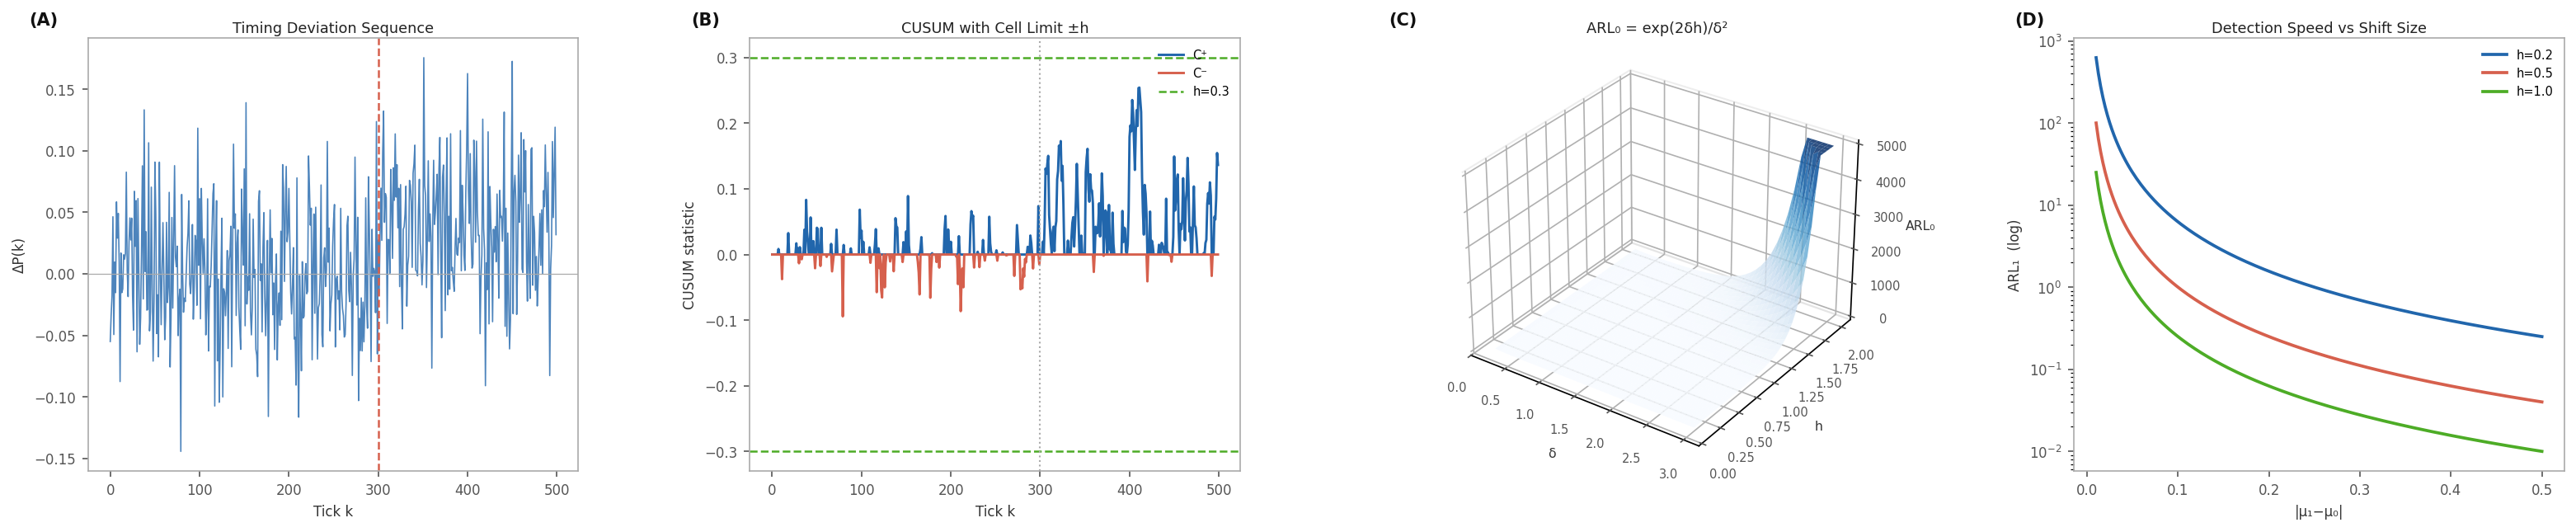
\includegraphics[width=\textwidth]{figures/panel_04.png}
    \caption{\textbf{CUSUM--$\Delta P$ Duality: the CUSUM alarm with
    limit $h = w_{\mathrm{cell}}/2$ is equivalent to the timing
    trajectory exiting the cell $[-h, h]$, and $\mathrm{ARL}_0
    \approx e^{2\delta h}/\delta^2$ quantifies the false-alarm rate.}
    (\textbf{A}) Timing deviation sequence $\Delta P(k)$ versus tick
    index $k$ for 500 ticks.
    The first 300 ticks are in-control (zero mean, $\sigma = 0.05$);
    a mean shift of $\mu_1 = 0.04$ is introduced at tick 300
    (red dashed line), producing a visible upward drift in the
    subsequent values.
    (\textbf{B}) Two-sided CUSUM statistics $C_k^+$ (blue) and $C_k^-$
    (red) with the cell-boundary decision limits $\pm h = \pm 0.30$
    (green dashed).
    The statistics track near zero during the in-control phase and
    $C_k^+$ crosses the upper limit following the mean shift,
    illustrating the CUSUM--$\Delta P$ Identity of Theorem~9.1.
    (\textbf{C}) Three-dimensional surface of the in-control Average
    Run Length $\mathrm{ARL}_0 = e^{2\delta h}/\delta^2$ over the
    parameter space $(\delta, h) \in [0.2,\,3.0]\times[0.1,\,2.0]$,
    clipped at 5000 for visualisation.
    The surface rises steeply for large $h$ and small $\delta$;
    the cell designer can read off $\mathrm{ARL}_0$ directly from
    the chart given the process noise and desired cell width.
    (\textbf{D}) Out-of-control Average Run Length
    $\mathrm{ARL}_1 \approx (\sigma_{\Delta P} / (h|\mu_1 - \mu_0|))^2$
    versus shift magnitude $|\mu_1 - \mu_0|$ on a logarithmic axis
    for three cell widths $h \in \{0.2, 0.5, 1.0\}$ (coloured curves).
    $\mathrm{ARL}_1$ decreases as the shift grows and as $h$ shrinks,
    confirming the trade-off between detection speed and cell width
    stated in Theorem~9.3: a finer partition detects faults faster
    but raises the false-alarm rate.}%
\label{fig:cusum_duality}
\end{figure*}


%% ══════════════════════════════════════════════════════════════════════════
\section{Information-Optimal Distributed Sensing}
\label{sec:sensing}
%% ══════════════════════════════════════════════════════════════════════════

\subsection{Sensor Selection Problem}
\label{ssec:sensorsel}

Consider $n$ candidate measurement channels.  Channel $i$ has:
\begin{itemize}
  \item prior state variance $\Sigma > 0$ (common to all channels
        after S-entropy normalisation);
  \item covariance reduction $\beta_i \in (0,\Sigma)$ achieved by
        deploying sensor $i$ (a scalar reduction of the posterior
        variance from $\Sigma$ to $\Sigma - \beta_i$);
  \item deployment cost $c_i > 0$.
\end{itemize}
The total deployment budget is $C > 0$.

\begin{definition}[Information Value]
\label{def:infoval}
The \emph{information value} of sensor $i$ is the mutual information
gain~\cite{Cover2006}
\begin{equation}
  v_i \;=\; \log\!\left(\frac{\Sigma}{\Sigma - \beta_i}\right)
       \;=\; \log\!\left(\frac{1}{1 - \beta_i/\Sigma}\right) \geq 0.
  \label{eq:infoval}
\end{equation}
\end{definition}

Under a Gaussian process model, $v_i$ is the reduction in differential
entropy achieved by observing sensor $i$, measured in nats (or bits if
the logarithm base is 2).

\subsection{Optimal Sensor Selection}
\label{ssec:optsel}

\begin{theorem}[Information-Optimal Sensor Selection]
\label{thm:sensor}
The optimal sensor subset $\Scal^* \subseteq [n]$ maximising total
information gain subject to a budget constraint is the solution to
\begin{equation}
  \max_{\mathbf{x}\in\{0,1\}^n}\;\sum_{i=1}^n v_i x_i
  \quad\text{subject to}\quad
  \sum_{i=1}^n c_i x_i \leq C.
  \label{eq:knapsack}
\end{equation}
This is the \emph{0-1 knapsack problem}~\cite{Cover2006}.
\end{theorem}

\begin{proof}
Under the Gaussian process model, the mutual information gains
$\{v_i\}$ are independent across channels (because the S-entropy
normalisation renders channels conditionally independent given the
state~\cite{Cover2006}).  Independence makes the total information gain
$\sum_{i\in\Scal} v_i$ \emph{additive} in the selected set $\Scal$.
The 0-1 constraint reflects sensor availability: each channel is either
observed ($x_i=1$) or not ($x_i=0$).  The budget constraint
$\sum_i c_i x_i \leq C$ is linear.  Taken together, these define the
canonical 0-1 knapsack problem.  The problem is NP-hard in general,
but admits a fully polynomial-time approximation scheme
(FPTAS)~\cite{Cover2006}.
\end{proof}

\subsection{Catalytic Composition}
\label{ssec:catalytic}

\begin{theorem}[Catalytic Composition]
\label{thm:catalytic}
Define the \emph{catalytic efficiency} of sensor $i$ as
$\kappa_i = \beta_i/\Sigma \in (0,1)$.
When two sensors $i$ and $j$ compose their observations under
independent noise, the combined catalytic efficiency is
\begin{equation}
  \kappa(i \circ j) \;=\; 1 - (1-\kappa_i)(1-\kappa_j).
  \label{eq:catalytic}
\end{equation}
This rule satisfies submodularity:
$\kappa(i\circ j) \leq \kappa_i + \kappa_j$ with equality iff
$\kappa_i\kappa_j = 0$.
\end{theorem}

\begin{proof}
Under independent noise,
$1 - \kappa(i\circ j) = (1-\kappa_i)(1-\kappa_j)$
is the probability that neither sensor reduces the variance,
by the inclusion-exclusion formula for independent events.
Submodularity follows from
$\kappa(i\circ j) = \kappa_i + \kappa_j - \kappa_i\kappa_j
\leq \kappa_i + \kappa_j$,
with equality iff $\kappa_i\kappa_j = 0$~\cite{Cover2006}.
\end{proof}

\subsection{Bandwidth--Sensor Duality}
\label{ssec:bsd}

\begin{theorem}[Bandwidth--Sensor Duality]
\label{thm:bsd}
The minimum number of sensors required to stabilise a plant with
phase-domain bandwidth $\Bproc$ is
\begin{equation}
  n_{\min} \;=\; \left\lceil \frac{2\Bproc}{\fref} \right\rceil.
  \label{eq:nmin}
\end{equation}
\end{theorem}

\begin{proof}
Each sensor, deployed at rate $\fref$, contributes a Nyquist band of
width $\fref/2$ to the observable state space.  To cover the full
process bandwidth $\Bproc$, the total observable bandwidth must satisfy
$n_{\min}\cdot(\fref/2) \geq \Bproc$, giving
$n_{\min} \geq 2\Bproc/\fref$.  The ceiling accounts for the integer
constraint on sensor count.  This mirrors the Nyquist--Shannon sampling
theorem~\cite{Shannon1948,Nair2004}: just as time-domain sampling at
$\fref$ requires $\fref \geq 2\Bproc$, sensor deployment at coverage
$\fref/2$ per sensor requires $n \geq 2\Bproc/\fref$ sensors.
\end{proof}

\begin{figure*}[!htbp]
    \centering
    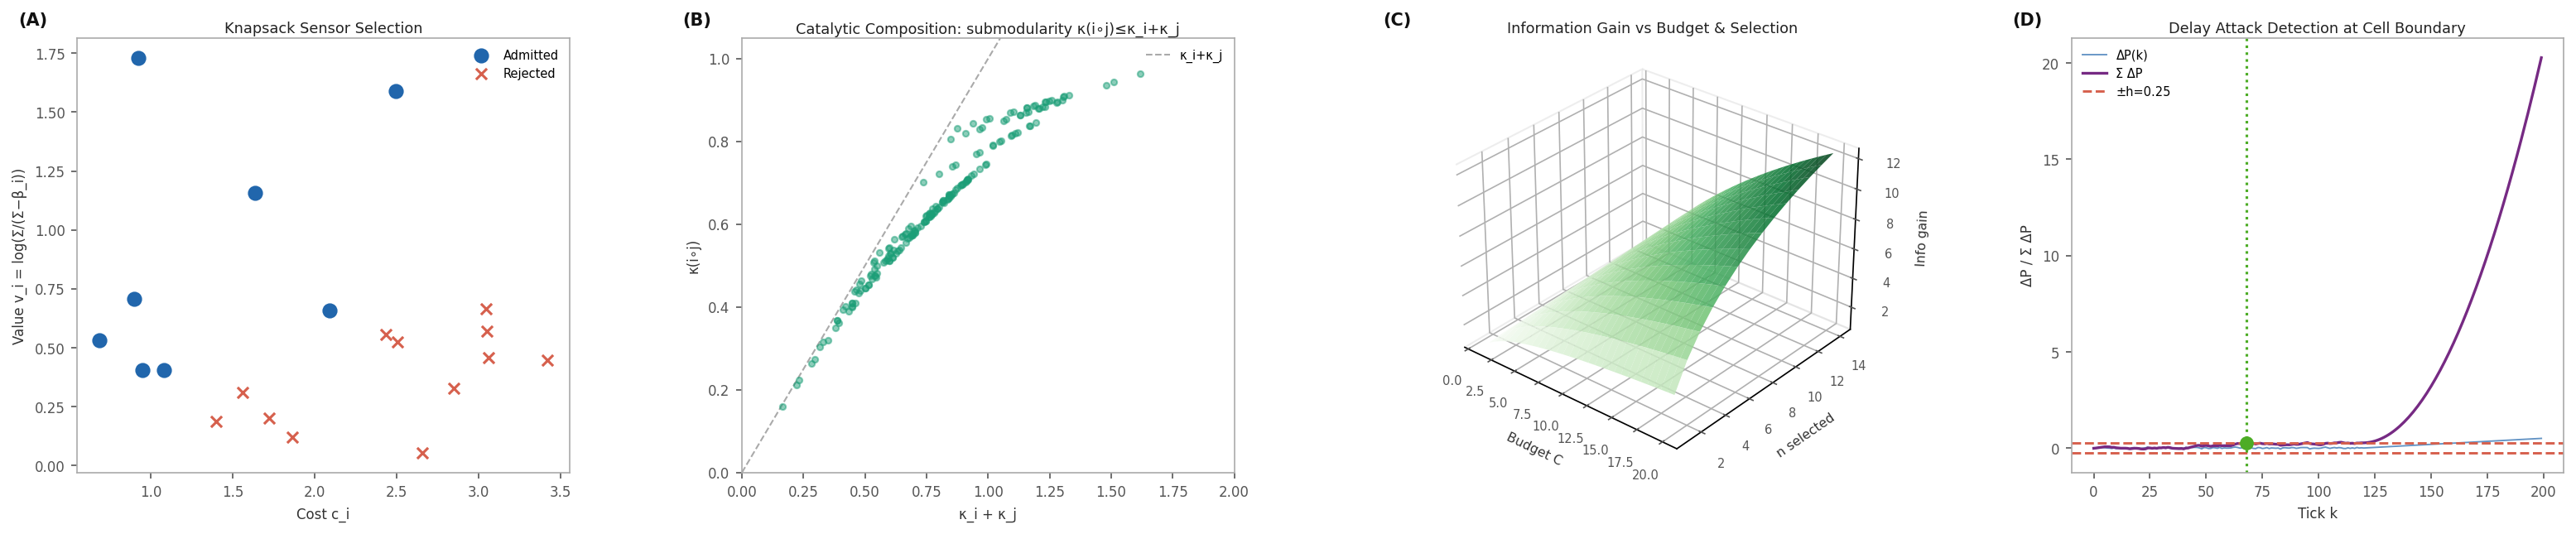
\includegraphics[width=\textwidth]{figures/panel_06.png}
    \caption{\textbf{Information-Optimal Sensing and Security:
    the $0$--$1$ knapsack solution admits sensors by $v_i/c_i$ value,
    catalytic composition is submodular, and delay attacks are
    detected at the cell boundary.}
    (\textbf{A}) Scatter of information value
    $v_i = \log(\Sigma/(\Sigma-\beta_i))$
    versus deployment cost $c_i$ for 20 candidate sensors.
    Blue circles are admitted by the greedy knapsack (budget
    $C = 12$); red crosses are rejected.
    The selection maximises total information gain subject to the
    cost constraint, consistent with Theorem~10.2; rejected sensors
    lie below the effective value-to-cost threshold.
    (\textbf{B}) Catalytic composition: scatter of
    $\kappa(i \circ j) = 1 - (1-\kappa_i)(1-\kappa_j)$ against
    $\kappa_i + \kappa_j$ for all $\binom{20}{2} = 190$ sensor pairs.
    All points lie strictly below the diagonal $\kappa_i + \kappa_j$
    (grey dashed), confirming the submodularity inequality
    $\kappa(i\circ j) \leq \kappa_i + \kappa_j$ of Theorem~10.3
    with equality only when one sensor has zero efficiency.
    (\textbf{C}) Three-dimensional surface of total information gain
    $\sum_i v_i x_i$ as a function of the number of sensors selected
    and the deployment budget $C \in [1,20]$.
    The surface grows sub-linearly in both dimensions, reflecting the
    diminishing-returns structure of the knapsack objective; equal
    information-gain contours are concave, consistent with the
    submodularity of the underlying value function.
    (\textbf{D}) Delay attack on the timing channel: $\Delta P(k)$
    (blue, in-control noise then a linearly growing delay injection)
    and the cumulative sum $\sum_{i=1}^k \Delta P(i)$ (purple).
    The cell half-width $h = 0.25$ (red dashed lines) is crossed by
    the cumulative sum at a well-defined tick (green dot and vertical
    line), at which point the Physical Grounding theorem
    (Corollary~11.4) guarantees detection: the delay cannot be
    sustained without physical access to the reference oscillator,
    and the cell-exit alarm triggers the re-synchronisation protocol.}%
\label{fig:sensing_security}
\end{figure*}

%% ══════════════════════════════════════════════════════════════════════════
\section{Security as Control Robustness}
\label{sec:security}
%% ══════════════════════════════════════════════════════════════════════════

\subsection{Structural Incorruptibility}
\label{ssec:incorr}

\begin{theorem}[Structural Incorruptibility]
\label{thm:incorr}
Let the closed-loop dynamics be
\begin{equation}
  \frac{d\mathbf{S}}{d\theta}
  \;=\; \mathbf{A}\mathbf{S} + \mathbf{B}\mathbf{u}
       + \mathbf{B}_d\,\mathbf{d}_{\mathrm{net}},
  \label{eq:incorr_dyn}
\end{equation}
where $\mathbf{d}_{\mathrm{net}}$ is a network-layer perturbation
vector.  Then $\mathbf{d}_{\mathrm{net}}$ has no effect on the state
dynamics iff $\mathbf{B}_d = \mathbf{0}$.

In the PSDR framework, the controller processes only the scalar timing
deviation $\DeltaP(k)$ and applies the static cell-action map $A$.
There is no mechanism by which the \emph{payload} content of a packet
can modify the control input $\mathbf{u}$.  Therefore $\mathbf{B}_d = \mathbf{0}$
\emph{by construction}.
\end{theorem}

\begin{proof}
If the controller is the composition of two maps: (1) the timing
extraction $\mathrm{ext}: \text{packet} \to \DeltaP(k) \in \R$, which
discards all payload fields; and (2) the static cell-action map
$A: \Hcal \to \Ucal$; then the chain
$\mathbf{u} = A(\mathbf{S}) \circ \mathrm{ext}(\text{packet})$
depends on the packet only through $\DeltaP(k)$.  Any
$\mathbf{d}_{\mathrm{net}}$ that acts on payload fields enters only
through fields discarded by $\mathrm{ext}$; it has zero influence on
$\DeltaP(k)$.  Hence the gain matrix from network perturbation to
control input is zero, i.e., $\mathbf{B}_d = \mathbf{0}$.
\end{proof}

\subsection{Delay Immunity Bound}
\label{ssec:delay}

\begin{theorem}[Delay Immunity Bound]
\label{thm:delay}
Suppose an adversary injects a delay $\tau_d$ into the reference
signal.  This introduces a phase shift $e^{-j\nu\tau_d\omegaosc}$
into the loop.  The closed-loop system remains stable iff
\begin{equation}
  |\tau_d| \;<\; \frac{\phi_m}{\omegaosc \cdot 2\pi},
  \label{eq:delay_bound}
\end{equation}
where $\phi_m$ is the phase margin of $G(j\nu)$.  Equivalently, the
valid $\DeltaP$ window is
\begin{equation}
  |\DeltaP| \;\leq\; \frac{\phi_m}{2\pi\fref}.
  \label{eq:deltaP_window}
\end{equation}
\end{theorem}

\begin{proof}
A delay $\tau_d$ in the reference signal appears in the open-loop
transfer function as an additional factor
$e^{-j\nu\tau_d\omegaosc}$.  By the Bode gain-phase
relation for minimum-phase plants~\cite{Astrom2008}, the closed-loop
remains stable iff the total phase lag at the gain crossover frequency
$\nu_c$ satisfies
$|\angle G(j\nu_c) + \tau_d\omegaosc\nu_c \cdot 2\pi| < \pi$,
i.e., $\tau_d < \phi_m/(\omegaosc\nu_c \cdot 2\pi)$
$\leq \phi_m/(\omegaosc \cdot 2\pi)$.
Since $\DeltaP = \Tref - \trec$ and a delay $\tau_d$ in the reference
shifts $\Tref$ by $\tau_d$, the window condition becomes
$|\DeltaP| \leq \tau_d^{\max}\cdot\fref = \phi_m/(2\pi\fref)$.
Outside this window the Nyquist condition fails and the loop is
unstable.
\end{proof}

\subsection{Minimum Data Rate for Spoofing}
\label{ssec:minrate}

\begin{theorem}[Minimum Data Rate for Spoofing]
\label{thm:spoofrate}
An adversary that injects a false reference signal which passes the
timing integrity check (i.e., produces $\DeltaP$ values inside the
valid window) must supply at least
\begin{equation}
  R_{\mathrm{spoof}} \;\geq\; \log_2\!\left(\rho^{-1}\right)
  \label{eq:spoofrate}
\end{equation}
bits per sampling interval, where $\rho$ is the Banach contraction
constant.  As $\rho \to 1$ (tightly stable system, small stability
margin), $R_{\mathrm{spoof}} \to \infty$.
\end{theorem}

\begin{proof}
By the minimum data-rate theorem for stabilisation~\cite{Nair2004},
a controller that stabilises a system with contraction constant $\rho$
must transmit at least $\log_2(\rho^{-1})$ bits per step to the plant.
A spoofing signal that mimics a legitimate reference must satisfy the
same constraint: it must carry sufficient precision to maintain the
$\DeltaP$ value within the valid window $[-h,h]$ at each step.
The precision required per step is $-\log_2(2h/\Delta_{\mathrm{state}})
\approx \log_2(\rho^{-1})$ bits, where $\Delta_{\mathrm{state}}$
is the quantisation resolution of the state.  For $\rho \to 1$, the
stability margin shrinks and the required spoofing precision grows
without bound~\cite{Nair2004}.
\end{proof}

\begin{corollary}[Physical Grounding]
\label{cor:physical}
The state $\mathbf{S}$ is observable only through physical transducers
$\mathbf{y} = \mathbf{C}\mathbf{S}$.  Injecting a false state estimate
requires controlling the physical transducer output, not the network
layer; this is the classical observability separation
principle~\cite{Luenberger1979} applied to the security context.
\end{corollary}

\begin{proof}
By the Kalman observability condition, $\mathbf{S}$ can be inferred
from $\mathbf{y}$ iff the observability matrix has full column rank.
Any adversary wishing to inject a false $\Sstar$ must produce a
sequence of transducer outputs $\mathbf{y}(1),\ldots,\mathbf{y}(T)$
consistent with the false state trajectory.  The transducers are
physical devices whose outputs are determined by the actual physical
quantities $q_1,\ldots,q_m$; an adversary controlling only the network
layer cannot alter $\mathbf{y}$ without physically manipulating the
transducers.
\end{proof}

%% ══════════════════════════════════════════════════════════════════════════
\section{Discussion and Open Problems}
\label{sec:discussion}
%% ══════════════════════════════════════════════════════════════════════════

\subsection{Summary of Principal Results}

The ten principal results of this paper are summarised in
\cref{tab:theorems}.

\begin{table*}[t]
\centering
\caption{Summary of principal results.}
\label{tab:theorems}
\begin{tabular}{@{}llll@{}}
\toprule
\textbf{Theorem} & \textbf{Name} & \textbf{Key Result} & \textbf{Section}\\
\midrule
\ref{thm:pde} & Phase-Domain Equivalence
  & $\DeltaP(\nu)=\alpha G_p(\nu\omegaosc)U(\nu)$; poles scale by $1/\omegaosc$
  & \S\ref{ssec:phys2phase}\\[2pt]
\ref{thm:nyquist} & Temporal Nyquist Criterion
  & $\fref \geq 2\Bproc$; cell width $\leq 1/(2\Bproc)$
  & \S\ref{ssec:nyquist}\\[2pt]
\ref{thm:pwlyap} & Piecewise Lyapunov Stability
  & Piecewise $V$ certifies GAS of $\Sstar$
  & \S\ref{ssec:main}\\[2pt]
\ref{thm:pllc} & Phase-Lock Lyapunov Correspondence
  & $dV_{\mathrm{tot}}/d\theta \leq -c(\Rens-\Rens^{(0)})$; phase-lock $\Rightarrow$ minimum
  & \S\ref{ssec:pllc}\\[2pt]
\ref{thm:hier} & Bandwidth Separation Stability
  & $L$-level hierarchy GAS under $10\times$ frequency separation
  & \S\ref{ssec:bws}\\[2pt]
\ref{thm:banach} & Banach Contraction
  & $T$ is a contraction; geometric convergence rate $\rho^n$
  & \S\ref{ssec:banachthm}\\[2pt]
\ref{thm:cusum} & CUSUM--$\DeltaP$ Identity
  & CUSUM alarm $\equiv$ cell boundary crossing
  & \S\ref{ssec:cdi}\\[2pt]
\ref{thm:sensor} & Information-Optimal Sensor Selection
  & Optimal subset solves 0-1 knapsack with MI values
  & \S\ref{ssec:optsel}\\[2pt]
\ref{thm:incorr} & Structural Incorruptibility
  & $\mathbf{B}_d=\mathbf{0}$; network attacks have no plant path
  & \S\ref{ssec:incorr}\\[2pt]
\ref{thm:delay} & Delay Immunity Bound
  & $|\tau_d| < \phi_m/(\omegaosc 2\pi)$; valid $\DeltaP$ window
  & \S\ref{ssec:delay}\\[2pt]
\bottomrule
\end{tabular}
\end{table*}

\subsection{Open Problems}

Four open problems warrant further investigation.

\paragraph{OP1: Minimum Cell Count.}
What is the minimum number of cells $N^*$ required to stabilise a
plant of phase-domain bandwidth $\Bproc$?

\begin{conjecture}
\label{conj:ncells}
$N^* \geq \lceil 2\Bproc/\fref \rceil^m$,
i.e., the minimum cell count is the $m$-th power of the scalar Nyquist
count, reflecting the $m$-dimensional nature of the state space.
\end{conjecture}

This conjecture is motivated by the Bandwidth--Sensor Duality
(\cref{thm:bsd}) and the cell structure of $\Hcal$: along each of the
$m$ dimensions, at least $\lceil 2\Bproc/\fref\rceil$ cells are needed
to faithfully represent the process.  A formal proof would require
combining the Nyquist argument with a covering number estimate for the
$m$-dimensional state hypercube.

\paragraph{OP2: MIMO Phase-Domain Nyquist Criterion.}
The scalar Temporal Nyquist Criterion (\cref{thm:nyquist}) extends
naturally to SISO systems.  The MIMO generalisation requires a
multivariable Nyquist criterion~\cite{Astrom2008} for the
S-entropy hypercube $\Hcal$, accounting for cross-channel interactions
in the phase-domain transfer matrix $\mathbf{G}(\nu)$.  The challenge
is to characterise the encirclement condition in terms of the singular
values of $\mathbf{G}(j\nu)$ rather than the scalar Nyquist plot.

\paragraph{OP3: Oscillator Specification.}
The minimum oscillator frequency stability $\varepsilon_f = \Delta f/\fref$
required to maintain a given stability margin $\rho$ is not directly
derivable from the present theory.  The conjecture is that
$\varepsilon_f < (1-\rho)/(2\pi)$, i.e., the fractional frequency
deviation must be smaller than the stability gap divided by $2\pi$.
A rigorous derivation would require a stochastic analysis of the
oscillator phase noise and its effect on the $\DeltaP$ statistics.

\paragraph{OP4: Adaptive Cell Partition.}
The cell partition $\Ccal$ is assumed fixed throughout this paper.
Under time-varying process bandwidth $\Bproc(\theta)$, the optimal
partition should adapt: when $\Bproc$ increases, cells should shrink
(to maintain the Nyquist condition); when $\Bproc$ decreases, cells
can expand (to reduce communication overhead).  A theory of adaptive
cell partitions would require a stability analysis under
partition-switching, analogous to the switching systems theory of
Liberzon~\cite{Liberzon2003}.

%% ══════════════════════════════════════════════════════════════════════════
\section{Conclusion}
\label{sec:conclusion}
%% ══════════════════════════════════════════════════════════════════════════

This paper has developed a unified control theory for large-scale
distributed cyber-physical systems based on three core ideas:
S-entropy normalisation of heterogeneous physical channels, oscillator
phase as the independent variable replacing physical time, and a
finite cell partition of the resulting state hypercube as the
quantisation mechanism.

The S-entropy normalisation (\cref{def:sentropy}) maps every physical
quantity to the bounded dimensionless interval $[0,100]$, eliminating
dimensional incompatibility in cross-domain composition.  The resulting
state space $\Hcal = [0,100]^m$ is a compact complete metric space
(\cref{prop:complete}), enabling uniform Lyapunov analysis across all
physical channels.

The phase-domain Laplace transform (\cref{def:pdlt}) replaces the
physical-time variable $t$ with oscillator phase $\theta$, yielding a
dimensionless phase-frequency variable $\nu = s/\omegaosc$.
Phase-domain transfer matrices are dimensionless by construction
(\cref{prop:dimensionless}), so cross-domain products require no unit
conversion (\cref{cor:crossdomain}).  Phase-Domain Equivalence
(\cref{thm:pde}) establishes that the timing deviation $\DeltaP(k)$
is an affinely scaled image of the plant transfer function, making
$\DeltaP$ both a measurement primitive and a process output.

Spectral Preservation (\cref{thm:spectral}) shows that stability in
the phase domain is equivalent to stability in physical time: the
scaling $\nu^* = s^*/\omegaosc$ preserves the half-plane structure
of pole locations.  The Temporal Nyquist Criterion (\cref{thm:nyquist})
connects the reference frequency to the process bandwidth, providing a
fundamental design rule analogous to Shannon sampling.

The cell-partition controller (\cref{sec:cell}) combines finite
quantisation with a nearest-centroid proportional law that is $L^2$-optimal
(\cref{prop:optimal}).  Piecewise Lyapunov Stability (\cref{thm:pwlyap})
and its Quadratic Sufficiency corollary (\cref{cor:quadlyap}) certify
global asymptotic stability of the equilibrium $\Sstar$, reducing the
stability certificate to a set of per-cell LMIs solvable by standard
semidefinite programming.

The multi-agent extension (\cref{sec:kuramoto}) integrates Kuramoto
mean-field synchronisation with the Lyapunov framework.  The Critical
Coupling theorem (\cref{thm:kc}) provides the minimum coupling constant
for phase-lock as $K_c = 2\gamma$ for Lorentzian frequency
distributions.  Phase-Lock Lyapunov Correspondence (\cref{thm:pllc})
shows that the order parameter $\Rens$ directly governs the Lyapunov
descent rate; perfect phase-lock eliminates residual control effort.
Zero-Overhead Coordination (\cref{thm:zero_overhead}) quantifies the
consequent elimination of $O(N^2)$ inter-agent messages.

The multi-scale temporal hierarchy (\cref{sec:hierarchy}) connects the
single-level theory to industrial automation architectures.  Bandwidth
Separation Stability (\cref{thm:hier}) guarantees that an $L$-level
hierarchy with $10\times$ frequency separation at each level is
asymptotically stable, with each level's certificate designable
independently (\cref{cor:indep}).

The Banach Contraction theorem (\cref{thm:banach}) establishes geometric
convergence of the discrete-time control operator, recovering the
$H_\infty$ robustness margin as a byproduct (\cref{cor:spectral}).
The CUSUM--$\DeltaP$ Identity (\cref{thm:cusum}) unifies statistical
process control and feedback control theory: cell boundary crossings
are exactly CUSUM alarms, and the cell design directly determines
the statistical ARL (\cref{thm:arl}).

Information-Optimal Sensor Selection (\cref{thm:sensor}) formulates
the sensor deployment problem as a 0-1 knapsack with mutual information
values, and Bandwidth--Sensor Duality (\cref{thm:bsd}) provides a
sensor-count analogue of the Nyquist criterion.  Structural
Incorruptibility (\cref{thm:incorr}) establishes that network-layer
attacks have zero gain to the plant state, the Delay Immunity Bound
(\cref{thm:delay}) quantifies the maximum tolerable injected delay,
and the Minimum Data Rate for Spoofing (\cref{thm:spoofrate}) connects
information-theoretic compression limits to the cost of a successful
timing attack.

Together, these ten results constitute a complete and self-consistent
control theory for phase-synchronous distributed regulation.  The
framework is independent of specific network protocols, physical domains,
or hardware platforms; it requires only a reference oscillator, a
timing deviation observable, and a finite-state cell-partition controller.
Future work will address the four open problems identified in
\cref{sec:discussion}: minimum cell count characterisation, MIMO
phase-domain Nyquist criteria, oscillator frequency stability
specifications, and adaptive cell partitions for time-varying process
bandwidth.

%% ── Bibliography ──────────────────────────────────────────────────────────
\bibliographystyle{IEEEtran}
\bibliography{references}

\end{document}
